\documentclass{book}

\usepackage{tikz}
\usepackage[compat=1.1.0]{tikz-feynman}
\usetikzlibrary{angles, quotes}
\usetikzlibrary{calc}
\usetikzlibrary{external}
\usetikzlibrary{decorations.pathreplacing, shapes.misc}
\usetikzlibrary{decorations.markings}
\tikzexternalize[prefix=tikz/]
\tikzset{external/system call={lualatex \tikzexternalcheckshellescape -halt-on-error -interaction=batchmode -jobname "\image" "\texsource"}}
\usepackage{shellesc}
\usepackage{subcaption}


\usepackage[backend=biber, style=apa]{biblatex}  
\addbibresource{biblio.bib}


\usepackage[english]{babel}
\usepackage[a4paper]{geometry}
\usepackage{pgfplots}
\pgfplotsset{compat=1.17} 
\usepgfplotslibrary{fillbetween}

\usepackage{csquotes}
\usepackage{array}
\usepackage{multirow}
\usepackage{enumitem}
\usepackage[normalem]{ulem}
\usepackage{tabularx}
\usepackage{amsmath}
\usepackage{amssymb}
\usepackage{amsfonts}
\usepackage{physics}
\usepackage{graphicx}
\usepackage[colorlinks=true, allcolors=blue]{hyperref}
\usepackage{lineno}
\usepackage{xspace}


\newcommand{\Ms}[0]{\textup{M}_\odot}
\newcommand{\todo}[1]{{\textcolor{red}{\bf \large #1}}}
\newcommand{\consignes}[1]{{\textcolor{blue}{\bf \large #1}}}

\def\lemaitre{\textsc{Lemaître}\xspace}
\def\skysurvey{\texttt{skysurvey}\xspace}
\def\pets{\texttt{PETS}\xspace}
\def\nacl{\texttt{NaCl}\xspace}
\def\edris{\texttt{EDRIS}\xspace}
\def\saltd{\texttt{SALT2.4}\xspace}



\let\mcl\mathcal
\let\ov\overline
\let\ra\rightarrow

\newcolumntype{C}{>{\centering\arraybackslash}X}

\title{Rapport final de stage de Recherche au LPNHE\\\vspace{.3em} \large Mesure de la croissance des structures avec les galaxies du DESI BGS et les supernovae de type Ia de ZTF~: vers une analyse jointe}
\author{Antoine Gilles--Lordet\\ \vspace{.1em} \small encadré par Pauline Zarrouk et Nicolas Regnault }
\date{}

\begin{document}

\maketitle

\tableofcontents

\chapter{Synthèse}

\consignes{Une synthèse d’une page (ou executive summary) présentant le problème posé et ses enjeux pour le client, les éléments clés de la démarche, les solutions apportées et les résultats obtenus, et ce, en français et en anglais}

La cosmologie moderne repose sur un modèle nommé $\Lambda$CDM, construit à partir de la relativité générale d'Albert Einstein, et supposant que l'univers contient environ 5\% de matière ordinaire, 25\% de matière noire qui n'interagit que gravitationnellement, et de 60\% d'énergie noire dont le rôle est d'accéléré l'expansion de l'Univers. Cette accélération est encore mal comprise, et des modèles alternatifs de gravitation l'explique sans faire intervenir cette dernière composante. Dans ce contexte, ce stage vise à déterminer le taux de croissance des structures dans l'Univers, car l'évolution temporelle de cette grandeur dépend directement du modèle considérée. Elle constitue donc un test de la relativité générale aux échelles cosmologiques.

Ce stage se base sur les données de deux relevés, le relevé \textit{Dark Energy Spectroscopic Instrument} (DESI) et le relevé \textit{Zwicky Transient Facility} (ZTF). DESI a pour objectif de cataloguer et cartographier les galaxies de notre Univers proche, en mesurant leurs positions angulaires et leur redshift par spectroscopie. Ces galaxies possèdent une vitesse propre par rapport à l'expansion de l'Univers car elles sont constamment attirées par les puits de potentiels gravitationnels. Ces vitesses particulières déforment alors la distribution des redshift par effet Doppler, et il est possible de mesurer le taux de croissance des structures à partir de cette distorsion. ZTF est quand à lui un programme d'observation visant à détecter les phénomènes transitoires, en particulier les \textit{supernovae} (SN) de type Ia. Ces SNe sont particulièrement intéressante puisqu'elles constituent des chandelles standards, c'est-à-dire que leurs luminosités et leurs distances sont corrélées, ce qui permet de reconstruire avec précision la vitesse de leur galaxies hôtes. Leur utilisation en combinaison avec un catalogue de galaxies permet d'améliorer considérablement la précision sur la mesure du taux de croissance des structures.

Lors de ce stage, j'ai assemblée une chaîne d'analyse cosmologique et je l'ai testée sur des simulations. Pour cela des SNe possédant des vitesses particulières sont générées selon un modèle cosmologique fixé, et des observations sont simulées à l'aide des logs d'observations de ZTF. La chaîne d'analyse permet alors de reconstruire les paramètres de ces SNe ainsi que leurs vitesses particulières, afin d'en déduire le taux de croissance des structures.

\chapter{Introduction}

\section{Contexte}

Le modèle standard de la cosmologie, nommé $\Lambda$CDM, suppose que la gravité est décrite à toutes les échelles par la relativité générale, et que les principales contributions à la gravité viennent de la matière noire froide (\textit{Cold Dark Matter}) et l'énergie noire (sous la forme d'une constante cosmologique $\Lambda$). Ces deux inconnues sont nécessaires pour décrire l'évolution de l'Univers ainsi que la croissance des structures aux grandes échelles, et permettent à ce jour de reproduire fidèlement les observations, en particulier l'expansion accélérée de l'Univers. Cependant des modèles alternatifs de gravité ont également été proposés pour expliquer cette accélération sans faire intervenir de constante cosmologique, et prédisent des évolutions temporelles différentes de celles de la relativité générale pour certaines quantités.

Parmi ces quantités, on trouve notamment le taux de croissance des structures en fonction du redshift\footnote{En français, \textit{décalage vers le rouge}, effets de dilatation des longueurs d'ondes des photons entre leur émission et leur observation sur Terre du à l'expansion de l'Univers. Le terme anglais sera utilisé plutôt que sa traduction pour alléger les propos.} $f(z)$, et l'écart-type du champ de densité dans une sphère de rayon 8$h^{-1}$Mpc, $\sigma_8$. Ces deux quantités sont intéressantes car on peut montrer les vitesses particulières des galaxies, c'est-à-dire leurs vitesses par rapport à l'expansion de l'univers, sont proportionnelles au produit $f(z)\sigma_8(z)$ et caractérisent ainsi la formation des structures observées dans l'univers.

En plus de la nature inconnue de la matière noire et de l'énergie noire, le modèle $\Lambda$CDM présente également des tensions sur certains paramètres. Une tension survient lorsque des analyses utilisant différents types d'observation obtiennent une différence significative de valeur de paramètres. La plus connue est la tension sur la constante de Hubble $H_0$\footnote{les mesures directes utilisant le fond diffus cosmologique donne $H_0 \sim 67$ km.s$^{-1}$.Mpc$^{-1}$, tandis que les mesures indirectes reposant sur des supernovae ou des phénomènes de lentillage gravitationnel tendent vers $H_0 \sim 73$ km.s$^{-1}$.Mpc$^{-1}$.}, mais il existe également une tension sur $\sigma_8$ (voir les valeurs en Table \ref{tab:fs8}. Il est donc particulièrement important de déterminer sa valeur avec précision.

\begin{table}
	\begin{tabular}{l|c}
		Relevé & valeur\\
		\hline\\
		Planck2018 (\cite{planck_collaboration_planck_2020}) & $\sigma_8 = 0.811\pm 0.006$\\
		DES Y3 + KIDS-1000 (\cite{dark_energy_survey_y3_2023}) & $\sigma_8 = 0.825^{+0.067}_{-0.073}$\\
		SDSS IV  (\cite{eboss_collaboration_completed_2021}) & $\sigma_8 = 0.85 \pm 0.03$\\
		DESI (\cite{chen_not_2024}) & $\sigma_8 = 0.878^{+0.089}_{-0.080}$
	\end{tabular}
	\caption{Mesures de $\sigma_8$ avec différentes sondes}
	\label{tab:fs8}
\end{table}

\subsection{Analyse du clustering des galaxies pour mesurer $f\sigma_8$}

Pour mesurer la croissance des structures, la méthode la plus commune se base sur les \textbf{\textit{Redshift Space Distorsion} (RSD)} (\cite{kaiser_clustering_1987}), des distorsions liées aux transformations des coordonnées comobiles vers l'espace des redshifts. Le redshift mesuré, par exemple par spectroscopie, ne contient pas uniquement le redshift cosmologique dû à l'expansion de l'univers, mais inclut également une contribution par effet Doppler due aux vitesses particulières des galaxies, c'est-à-dire leurs vitesses propres par rapport à l'expansion de l'Univers.

Ce terme supplémentaire déplace les galaxies dans l'espace des redshifts par rapport à l'espace comobile, et les corrélations spatiales du champ de densité deviennent alors anisotropes : le long de la ligne de visée, les galaxies semblent plus regroupées qu'orthogonalement à la ligne de visée. A grande échelle, l'amplitude de cette anisotropie étant proportionnelle au facteur de croissance des structures $f$ et à l'amplitude des fluctuations du champ de densité, représenté communément par $\sigma_8$ (l'écart-type du champ de densité dans une sphère de rayon 8$h^{-1}$Mpc), ces analyses du clustering des galaxies contraignent le paramètre composite $f(z)\sigma_8(z)$. De nombreuses analyses des distorsions dans l'espace des redshifts ont été effectuées à l'aide de relevés spectroscopiques, tels que 6dFGRS (\cite{beutler_6df_2012}), SDSS-MGS (\cite{howlett_clustering_2015}), FastSound (\cite{okumura_subaru_2016}), SDSS-III BOSS (\cite{alam_clustering_2017}) ou SDSS-IV eBOSS (\cite{eboss_collaboration_completed_2021}). Les dernières mesures atteignent une précision de l'ordre de 10\%, et sont compatibles avec la relativité générale.

Une autre méthode pour mesurer $f\sigma_8$ est de dériver le paramètre des mesures directes des vitesses particulières des galaxies. Les vitesses particulières peuvent être mesurées directement à condition de pouvoir mesurer indépendamment les redshifts et les distances absolues des galaxies. Des mesures précises des redshifts peuvent être obtenues par spectroscopie et des estimations des distances peuvent être obtenues en utilisant les corrélations entre les distances et d'autres observables, telle que la relation de Tully-Fisher pour les galaxies spirales (corrélation entre la vitesse radiale de ses étoiles et la luminosité totale de la galaxie, \cite{tully_new_1977}) ou la méthode du Plan Fondamental (\cite{djorgovski_fundamental_1987}). Ces corrélations sont utilisables uniquement pour des galaxies à des redshifts relativement faibles ($z < 0,1$) car les incertitudes augmentent rapidement avec le redshift. Les propriétés statistiques d'un échantillon de vitesses particulières peuvent ensuite être utilisées seules ou en combinaison avec un champ de densité de galaxies (\cite{adams_joint_2020, qin_redshift_2019, turner_local_2023}.

\subsection{DESI}

De telles analyses font parties des objectifs du relevé \textit{Dark Energy Spectrscopic Instrument} (DESI). Ce programme d'observation utilise 5000 fibres optiques positionnées par robots pour réaliser des spectres des galaxies nous entourant, afin de construire une cartographie 3D de l'univers proche, jusqu'à $z=1.7$. Ce relevé constitue le relevé de galaxies le plus dense jamais réalisées, les premières données publiées (nommées DESI EDR) représentent 700 000 objets, et seulement 1\% du volume final couvert. La publication des données DESI Y1\footnote{Lire \textit{DESI year one}, données dont la prise a été finalisée en juin 2022} est prévue pour 2025, mais a déjà permis la réalisation d'analyses cosmologiques (\cite{desi_collaboration_desi_2024, desi_collaboration_desi_2024-1, desi_collaboration_desi_2024-2}) ainsi que la production de catalogues simulés fidèles à l'univers observé, tel que le catalogue Uchuu.

Ce catalogue a été réalisé à partir de la simulation Uchuu (\cite{prada_desi_2023}), une simulation à N-corps utilisant 2.1 milliards de particules, peuplée avec des galaxies du \textit{DESI Bright Galaxy Survey} (BGS) qui est un set complet de galaxies lumineuses\footnote{ce sous-échantillon est défini comme ayant une magnitude en bande r inférieure à $19.5$} à bas redshift ($z<0.4$) (\cite{hahn_desi_2023}), pour produire un univers statistiquement fidèle au notre. Le catalogue ainsi obtenu reproduit le champ de densité de la simulation Uchuu mais aussi le champ de vitesse. Il donne donc accès aux redshifts cosmologiques et aux redshifts observés, et peut être utilisé comme base d'une analyse $f\sigma_8$ sur des simulations.


\subsection{Analyse cosmologique avec des SN Ia pour mesurer $f\sigma_8$}

À bas redshift, un autre moyen d'obtenir les distances vient des supernovae (SNe) de type Ia (\cite{hoyle_nucleosynthesis_1960}). Ces SNe sont des explosions thermonucléaire de naine blanche dans un système binaire, riches en carbone et oxygène, et présentent la particularité d’avoir des conditions d'explosions très similaires les unes aux autres. En particulier, les évolutions temporelles de leur luminosité dans leurs référentiels propres sont très similaires. Le maximum de flux émis, environ 5 milliards de fois plus que le soleil, est corrélé à leurs durées et leurs couleurs intrinsèque selon deux lois, communément appelées \textit{brighter-slower} et \textit{brighter-bluer}. Les SNe plus brillantes présentent une décroissance plus lente (donc durent plus longtemps), et présentent un décalage de leurs longueurs d'ondes émises vers le bleu, qui n'est pas du à un effet de redshift.

Grâce à ces deux corrélations, il est possible de décrire leurs flux maximaux à l'aide de deux paramètres, nommés \textit{stretch}\footnote{Comme pour le redshift, le paramètre de \textit{stretch} n'a pas d'équivalent français utilisé dans la communauté, le terme anglais sera donc employé à la place.} et couleur, et d'exprimer leur flux maximal en fonction d'un flux moyen et de contributions liées au stretch et à la couleur.

Cette caractéristique rend les SNe Ia standardisables et en fait d'excellentes chandelles standard~: des événements astrophysiques dont la luminosité peut être modélisée, ce qui permet d'en déduire directement leurs distances. Les SNe Ia ont ainsi permis la découverte de l'accélération de l'expansion de l'Univers (\cite{perlmutter_cosmology_1998, riess_observational_1998}).

Pour exprimer cette standardisation, il est plus commode de travailler avec des magnitudes plutôt que des flux, définies par $M=\log_{10}(\mcl f)$. La standardisation des SN Ia est alors décrite par la formule de Tripp (\cite{tripp_two-parameter_1998})
\begin{equation}
\label{eq:tripp}
    M^*_{b,SN} = M_b - \alpha x_{1,SN} + \beta c_{SN} + \sigma_{int}
\end{equation}
où $M^*_{b,SN}$ est la magnitude absolue\footnote{\textit{i.e.} dans le référentiel propre} en bande B de la SN, $x_{1,SN}$ son \textit{stretch} et $c_{SN}$ sa couleur. $M_b$ est la magnitude absolue moyenne à $c=0$ et $x_1=0$ dans la bande B. Expérimentalement, on mesure $M_b=19.3$, ainsi que les coefficients $\alpha=0.14$ et $\beta=3.15$. En réalité, la standardisation n'est pas parfaite et une dispersion intrinsèque subsiste, représentée par $\sigma_{int}$. Cette dispersion est modélisée par une distribution gaussienne d'écart type $0.10$.

L'outil principal pour exploiter les SNe est le diagramme de Hubble, la représentation de la relation entre les distances des SNe, représentées par leurs magnitudes, avec leurs vitesses, représentée par leurs redshifts. Un tel diagramme est représenté en Figure \ref{fig:residues}. Un modèle peut alors être ajusté, et les résidus au modèle donnent accès aux vitesses particulières des SNe (\cite{davis_effect_2011}). En effet, les magnitudes des SNe dépendent de leurs redshift cosmologiques, dus à l'expansion de l'univers, et non de leurs redshift observé, qui inclue les vitesses particulières. Les SNe apparaissent alors comme décalées horizontalement par rapport au diagramme de Hubble, et leurs vitesses particulières sont contenues dans les résidus au modèle.

\begin{figure}
    \centering
    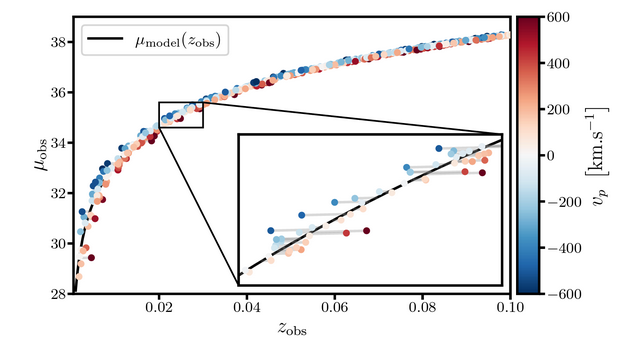
\includegraphics[width=0.8\textwidth]{figures/Residues.png}
    \caption{Diagramme de Hubble de SNe simulés. Les vitesses particulières selon la ligne de visée provoque un écart entre leur redshift cosmologique et le redshift observé, ce qui se traduit par un décalage horizontal des SNe par rapport à la ligne de base du diagramme de Hubble. Les SNe ayant une vitesse particulière positive s'éloignent de nous et nous apparaissent plus rouges, tandis que celles ayant une vitesse particulière négative nous apparaissent plus bleues. Crédit : B. Carreres}
    \label{fig:residues}
\end{figure}

Les analyses de clustering de galaxies sont moins performantes à bas redshift, car le volume étudié ne contient qu'un faible nombre de galaxies et cette statistique est insuffisante pour produire des analyses précises. Les SNe Ia constituent alors un bien meilleur traceur du champs de vitesses à bas redshift que les galaxies, et permettent de meilleurs contraintes sur la croissance des structures (cf Figure \ref{fig:fs8}).

\begin{figure}
    \centering
    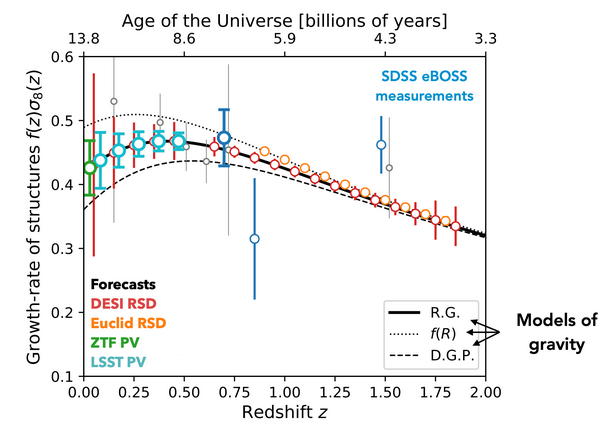
\includegraphics[width=0.8\textwidth]{figures/fs8.png}
    \caption{Prévisions des contraintes sur $f\sigma_8$ pour les relevés DESI (\cite{hahn_desi_2023}), Euclid (\cite{euclid_collaboration_euclid_2024}) et la combinaison de DESI avec des vitesses particulières de ZTF (\cite{carreres_growth-rate_2023}) ou LSST (\cite{howlett_2mtf_2017}). Credit : J. Bautista}
    \label{fig:fs8}
\end{figure}

\subsection{Le projet \lemaitre}

 La réalisation d'un diagramme de Hubble de nouvelle génération utilisant des lots encore non exploités de SN Ia des relevés \textit{Zwicky Transient Facility} (ZTF, \cite{bellm_zwicky_2018}), SuperNovae Legacy Survey (SNLS, \cite{pritchet_snls_2004}) et Hyper Suprime-Cam Subaru Strategic Programm (HSC-SSP, \cite{miyazaki_hyper_2012,aihara_hyper_2018}) est actuellement l’objet du projet \lemaitre au LPNHE. Ce projet vise à développer un nouveau pipeline d'analyse cosmologique des SN Ia à partir de zéro, adapté au traitement des volumes de données attendus des prochains programmes d’observation tels que LSST (\cite{the_lsst_dark_energy_science_collaboration_lsst_2021}). Le lot ZTF est appelé DR2.5, pour \textit{Data Release 2.5}, car il couvre les deux premières années de ZTF en prenant en compte des effets des capteurs jusqu'à présent inconnus. Ce projet utilisant des lots non exploités, la mesure des paramètres du modèle sera donc indépendante des mesures précédentes.

La partie analyse cosmologique du pipeline \lemaitre \footnote{Un module de calibration est présent en amont, mais n'est pas l'objet de ce stage et ne sera donc pas abordé.} (voir également la Figure \ref{fig:lemaitre_pipeline}) est composé des modules suivants~:
\begin{enumerate}
    \item Le module \pets (Preprocessing and sElection of a Training Sample) effectue une première sélection en éliminant les points de photométrie ainsi que les SNe mal échantillonnée. Il donne également une première évaluation des paramètre de standardisation des SNe, qui sert de point de départ pour NaCl. La principale difficulté que doit résoudre ce module est de proposer une sélection indépendante du redshift et du rapport signal sur bruit, car cela introduirait des biais dans la suite de l'analyse. Plus de détails sont disponibles en Annexe \ref{anx:pets}.
    \item Le module \nacl (Nouvel algorithme de Courbe de lumière) évalue ensuite les luminosités des SNe dans leurs référentiels propres, ainsi que leurs paramètres de standardisations en entraînant un modèle empirique. Il vise à ré-implémenter un modèle type \saltd ( adapté à l'analyse des volumes de données des relevés futures. De plus, les incertitudes sont propagées lors de l'entraînement, et ne nécessite pas leurs caractérisations a posteriori sur des simulations. Le fonctionnement détaillé de ce module est présenté en Annexe \ref{anx:nacl}.
    \item Le module \edris (Estimateur de Distance pour les Relevés Incomplets de Supernovae) utilise les paramètres de standardisations et leur matrice de covariance pour ajuster un modèle cosmologique, en prenant en compte des effets de sélection de manière analytique. Là encore, l'estimation des biais introduit par des effets de sélections sur les modèles est habituellement traitée a posteriori sur des simulations. Le détail de ce module est présenté en Annexe \ref{anx:edris}.
\end{enumerate}

Un des objectifs à long terme du projet \lemaitre qui guide le développement des modules est de disposer d'un pipeline d'intégration continue. Cela signifie qu'un module doit à terme pouvoir être modifié ou remplacé, et qu'une nouvelle analyse cosmologique complète doit pouvoir automatiquement être réalisée. L'ambition est d'ainsi pouvoir continuer à développer les modules existants, en prenant en compte différents effets ou biais et d'obtenir rapidement une estimation des gains et des biais potentiels sur les paramètres cosmologiques.

\begin{figure}
\centering
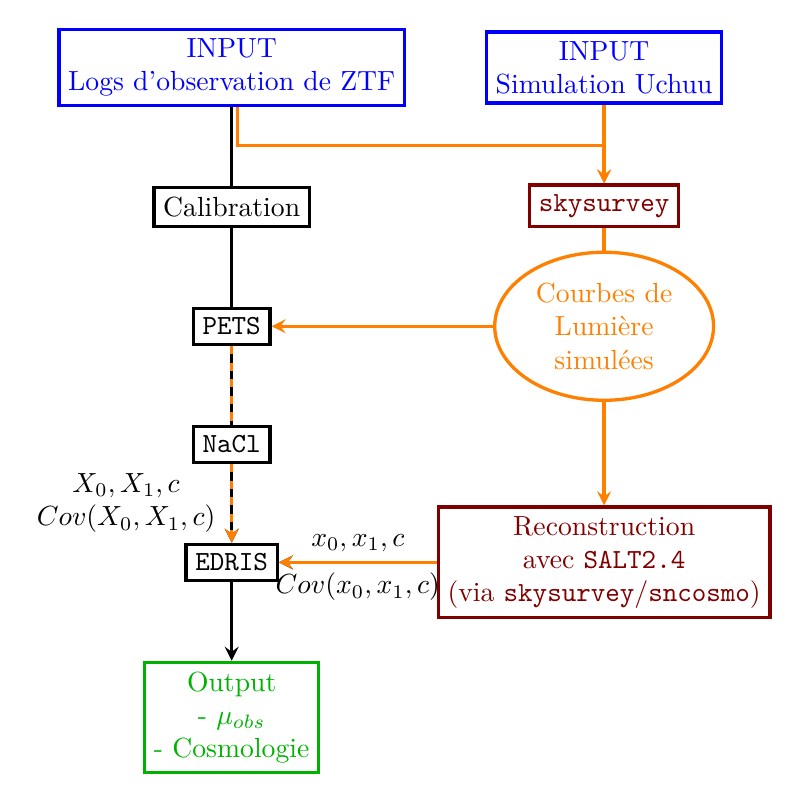
\begin{tikzpicture}[-stealth, line width=1.2pt]
	\node[rectangle, draw] (calib) at (0,0) {Calibration};
	\node[rectangle, draw, below=of calib] (pets) {\pets};
	\node[rectangle, draw, below=of pets] (nacl) {\nacl};
	\node[rectangle, draw, below=of nacl] (edris) {\edris};
	\node[rectangle, draw, below=of edris,  align=center, color=green!70!black] (out) {Output \\ - $\mu_{obs}$ \\ - Cosmologie};
	
	\node[rectangle, draw, above=of calib, color=blue, align=center] (logs) {INPUT \\ Logs d'observation de ZTF};	
	\node[rectangle, draw, right=of logs, color=blue, align=center] (uchuu) {INPUT \\ Simulation Uchuu};
	\node[rectangle, draw, below=of uchuu, red!50!black] (skys) {\skysurvey};

	\draw (logs) -- (calib) -- (pets) -- (nacl) -- (edris) node[left=2pt, pos=0.5, align=center, black] {$X_0, X_1, c$ \\ $Cov(X_0,X_1,c)$};
	\draw (edris) -- (out);

	\begin{scope}[orange]
		\draw [dashed] (pets) -- (nacl) -- (edris);
		\path (logs) -- (skys) coordinate[pos=0.5] (A);
		\draw ([xshift=2pt]logs.south) |- (A) -| (skys);
		\draw (uchuu) -- (skys);
		\node[ellipse, draw, align=center, aspect=2] (lcsim) at (skys |- pets) {Courbes de \\ Lumière \\ simulées};
		\draw (skys) -- (lcsim) -- (pets);
	\end{scope}
	\node[rectangle, draw, align=center, red!50!black] (rec) at (lcsim |- edris) {Reconstruction \\ avec \saltd \\ (via \skysurvey/\texttt{sncosmo})};
	\draw (rec) edge node[above, align=center] {$x_0,x_1,c$} node[below, align=center] {$Cov(x_0,x_1,c)$} (edris);
	\draw[orange] (lcsim) -- (rec);
	\draw[orange] (rec) -- (edris);
\end{tikzpicture}
\caption{Chaîne d'analyse \lemaitre développée au LPNHE (représentée en noire), et travail d'intégration effectué (en orange). L'étape de calibration contient en réalité plusieurs modules, mais elle n'a pas été utilisée pour ce stage car les données simulées n'incluait pas d'effets de calibration. \skysurvey ne fait pas partie intégrante de \lemaitre, il s'agit d'un sofware indépendant}
\label{fig:lemaitre_pipeline}
\end{figure}

\subsection{Analyse jointe }

Il est également possible de cumuler les deux analyses, en introduisant dans le clustering des galaxies les vitesses particulières des SNe. Une telle analyse $f\sigma_8$ a par exemple été menée dans \cite{boruah_bayesian_2022, stahl_peculiar-velocity_2021}. Ces analyses jointes permettent de meilleure contraintes sur $f\sigma_8$ à bas redshift que pour les analyses de RSD des galaxies seules (voir Fig. \ref{fig:fs8}), et sont donc particulièrement intéressante obtenir des mesure de précision.

\section{Objectifs}

L'objectif du stage est double~:
\begin{enumerate}
    \item Produire des échantillons simulés de SNe basés sur les positions des galaxies de la simulation Uchuu qui reproduit les données spectroscopiques du DESI BGS, ainsi que les observations de ZTF, et les utiliser pour tester le pipeline \lemaitre actuellement en développement au LPNHE pour produire les diagrammes de Hubble et reconstruire la cosmologie sous-jacente des échantillons. Le pipeline étant encore en développement, je développe l'intégration des différents modules et je les teste.
    \item Comparer les résultats de ce pipeline, \textit{i.e.} les positions ainsi que les vitesses particulières reconstruites, aux données d'entrée et les utiliser pour
    	\begin{enumerate}
		\item Estimer $f \sigma_8$ à partir des vitesses particulières de SNe de ZTF et comparer ces résultats avec ceux de B. Carreres (\cite{carreres_growth-rate_2023}).
		\item Produire une analyse jointe du DESI BGS et des SNe de ZTF pour quantifier le gain sur les contraintes de $f\sigma_8$.
	\end{enumerate}
\end{enumerate}

\section{Enjeux}

L'enjeu majeur de ce stage est la validation du pipeline \lemaitre sur des simulations. En particulier, l'intégration faisant partie des tâches de ce stage, les différents modules n'ont été testés qu'individuellement sur des données simplifiées ou approximées. Les simulations de SNe utilisées et passées à travers tous les modules sont plus réalistes et permettront de mettre en lumière les points critiques dans l'exécution du pipeline. Ces points critiques incluent (sans être restreints à) le paramétrage des modules, des différences éventuelles de convention ou de nommage des variables utilisées, des erreurs dans les modèles, approximations ou dans leur implémentation et la caractérisation des biais potentiels.
Le fait de travailler sur des simulations permet un plus fin contrôle des conditions de test que les données réelles, et de facilement prendre en compte ou retirer différents effets.

Un second enjeu est l'estimation du gain offert par \lemaitre, et plus généralement des SNe de ZTF, dans l'estimation de $f\sigma_8$ par rapport à une analyse du seul clustering du DESI BGS. Comme évoqué précédemment, la détermination précise de ce paramètre est essentielle pour pouvoir valider ou invalider différents modèles de gravitation.

\section{Reformulation du problème dans son contexte}

L'estimation précise du paramètre $f\sigma_8$ est essentielle à la cosmologie actuelle. Elle permet a minima de contraindre les paramètres du modèle $\Lambda$CDM, et de valider ou invalider différents modèles de gravités dont la relativité générale afin d'améliorer notre compréhension de l'Univers. Cette estimation nécessite, à bas redshift, l'utilisation de traceurs plus performants que les seuls catalogues de galaxie du fait du faible volume exploré. Les données de SNe Ia peuvent fournir les vitesses particulières nécessaires à cette estimation, mais les relevés récents et futurs nécessiteront de traiter des volumes de données plus importants qu'auparavant. Dans ce contexte, le développement d'une nouvelle chaîne d'analyse adaptée est fondamental, et est l'objectif du pipeline \lemaitre. Ce pipeline nécessite cependant d'être testé sur des simulations afin de diagnostiquer d'éventuels problème ou biais, et de quantifier la précision sur les vitesses particulières reconstruites.


\chapter{Approche et analyse}

\section{État de l'art}
\consignes{méthodes, raisons des choix faits, analyses menées (état de l’art)}

\subsection{Mesurer $f\sigma_8$ avec le clustering des galaxies et les SN de type Ia}
\label{sec:art}
 Plusieurs méthodes ont été développées pour extraire des mesures du taux de croissance à partir de vitesses particulières~:
 \begin{itemize}
     \item la méthode dite du maximum de vraisemblance, où les champs de vitesse (et de densité) sont supposés être tirés de distributions Gaussiennes multivariées et sur lesquels un ajustement de $f\sigma_8$ est réalisé par maximum de vraisemblance (\cite{johnson_6df_2014, huterer_testing_2017, howlett_2mtf_2017, adams_joint_2020, lai_using_2022, carreres_growth-rate_2023});
     \item l'analyse de statistiques compressées à deux points telles que la fonction de corrélation à deux points, le spectre de puissance, ou les vitesses moyennes par paire sur lesquelles $f\sigma_8$ est ajusté (\cite{nusser_velocity-density_2017, dupuy_estimation_2019, qin_redshift_2019, turner_local_2023});
     \item la comparaison entre les vitesses observées et celles reconstruites à partir du champ de densité (\cite{davis_effect_2011, carrick_cosmological_2015, boruah_cosmic_2020, said_joint_2020, stahl_peculiar-velocity_2021}). En utilisant un modèle de gravitation, on peut exprimer le champ de vitesse à partir du champ de densité et du taux de croissance des structures. Cette relation peut alors être utilisée pour obtenir $f\sigma_8$ en faisant concorder les vitesse particulières observées et celles obtenues à partir du champ de densité;
     \item l'inférence dite \textit{fieldlevel}, qui consiste à retracer l'évolution complète de l'univers à partir de conditions initiales à l'aide d'un modèle, puis à comparer le résultat obtenu aux observations des champs de densité et vitesses, et rétro-propager les erreurs jusqu'au conditions initiales (\cite{boruah_bayesian_2022, prideaux-ghee_field-based_2023}). 
\end{itemize}

Un résumé des valeurs obtenues par ces diverses analyse est représenté en Fig. \ref{fig:carreres_11}. J'utilise pour l'analyse $f\sigma_8$ la méthode décrite dans \cite{boruah_cosmic_2020,stahl_peculiar-velocity_2021}, qui est de comparer les vitesses observées reconstruites avec des SN Ia aux vitesses déduites du champ de densité. Une description plus détaillée est donnée en Annexe \ref{anx:fs8}.

\begin{figure}
    \centering
    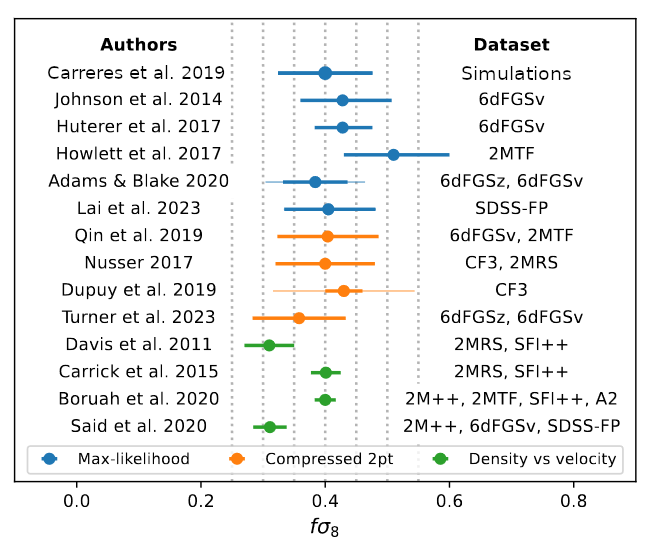
\includegraphics[width=0.7\textwidth]{figures/Carreres_fig_11.png}
    \caption{Mesures du coefficient de croissance des structures $f\sigma_8$ à partir de vitesses particulières et de catalogues de galaxies. Les barres d'erreurs en trait fin inclues les erreurs systématiques, à l'exception de Dupuy et al. 2019, pour lequel la contribution supplémentaire vient de la variance cosmique. Credit : 
    \cite{carreres_growth-rate_2023}.}
    \label{fig:carreres_11}
\end{figure}

\section{Approche de résolution du problème}
\consignes{présentation détaillée de l’approche de résolution de problème retenue, des ressources scientifiques, techniques et humaines mises en oeuvre, de l’organisation du travail}

La méthode employée pour la génération suit celle de \cite{carreres_growth-rate_2023} pour les simulations, c'est à dire de tirer les paramètres de standardisations de distributions expérimentales, puis de générer des observations à partir de ces paramètres et des logs d'observations réels de ZTF. La reconstruction de vitesses particulières des SNe utilisera elle les nouveaux modules développés pour le projet \lemaitre. L'analyse $f\sigma_8$ prévue suit quand à elle celle de \cite{boruah_cosmic_2020,stahl_peculiar-velocity_2021}.

\subsection{Génération des SN Ia}
\label{sec:gen_SN}

Les vitesses particulières des SNe simulées ne peuvent pas être tirées aléatoirement, puisqu'elles doivent être en accord avec les structures de galaxies et les unes avec les autres. Une possibilité est de simuler la dynamique de la matière noire d'un univers via une simulation à N-corps, et de la peupler de galaxies en fonction de la distribution de densité obtenue. 

Dans un premier temps, un échantillon de SN Ia est généré selon les distributions observées des paramètres $x_0$, $x_1$, $c$ et $t_0$ (voir Table \ref{tab:snia}), et les positions et redshifts des galaxies BGS simulées dans Uchuu à l'aide de \skysurvey\footnote{\href{https://skysurvey.readthedocs.io/en/latest/}{https://skysurvey.readthedocs.io/en/latest/}}.

\begin{table}
    \centering
    \begin{tabular}{p{6.5cm}|p{7cm}}
         Paramètre & Distribution \\
         \hline
         Temps de maximum du flux en bande B $t_0$ & Uniforme entre le 02/03/2018 et le 01/01/2021\\
         Stretch $x_1$ & Gaussienne bimodale (\cite{nicolas_redshift_2021})\\
         Couleur $c$ &  Loi exponentielle convoluée avec une gaussienne (\cite{ginolin_ztf_2024}) \\
         Magnitude absolue $m_{abs}$ & Obtenue par la formule de Tripp\\
         Magnitude observée $m_{obs}$ & $m_{obs} = 5 \log(d_L(z_{cosmo})) + 25 + m_{abs}$\\
         Amplitude $x_0$ & $x_0 = 10^{0.4(m_b - m_{obs})}$
    \end{tabular}
    \caption{Distributions utilisées pour le tirage des paramètres des SN Ia. Il est important de noter que le redshift utilisé pour le calcul des magnitudes observées utilise le redshift cosmologique, et non le redshift observé.}
    \label{tab:snia}
\end{table}

Seules les galaxies à redshift $z<0.06$ sont utilisées afin de s'affranchir du biais de Malmquist (voir notamment \cite{carreres_growth-rate_2023} ou \cite{boyd_accounting_2024}). Ce biais observationnel vient du fait que les télescopes ont une magnitude limite d'observation, au-delà de laquelle les SNe ne sont plus détectées. Or, à un redshift donné, les SNe couvrent une plage de magnitude du fait de la dispersion due aux paramètres de standardisations, à la dispersion intrinsèque et aux vitesses particulières. Ainsi, à haut redshift, les SNe les moins brillantes ne sont pas observées, ce qui biaiserait une estimation des paramètres cosmologique. ZTF est considéré complet jusqu'à $z=0.06$, ce qui signifie que l'impact du biais de Malmquist en dessous de ce redshift est négligeable.

La période du 02/03/2018 au 01/01/2021 utilisée pour le tirage du temps de maximum correspond à la plage temporelle de la DR2 de ZTF\cite{rigault_ztf_2024}. Cette restriction sert à la fois à avoir un volume de donné proche de celui que devra traiter le pipeline \lemaitre pour estimer sa rapidité, et à pouvoir quantifier le gain qui pourrait être obtenu sur $f\sigma_8$ avec des données réelles. Le taux d'explosions de SN Ia est pris égal à $2,35 .10^4$Gpc$^{-3}$ (\cite{perley_zwicky_2020}).
Pour le calcul de la magnitude observée, $d_L(z)$ représente la distance de luminosité, qui est calculée à l'aide d'un modèle $\Lambda$CDM contraint par les données de Planck 2015 (\cite{planck_collaboration_planck_2016}) pour correspondre au modèle cosmologique utilisé par la simulation Uchuu.

Une simulation du relevé SNLS est également réalisée afin d'avoir un échantillon de SNe à plus haut redshift pour mieux contraindre le modèle cosmologique. Comme les redshifts observés par SNLS vont environ de $z=0.1$ à $z=1.2$, ils sont trop élévés pour le catalogue Uchuu BGS. Les positions des SNe sont donc tirées uniformément dans la footprint SNLS, et n'incluent pas d'effets de vitesses particulières. Seule la simulation de ZTF sera utilisée pour la reconstruction des vitesses particulières.

\subsection{Reconstruction des vitesses particulières}

Une fois les paramètres tirés, des points de données d'observations photométriques et spectroscopiques sont générés en utilisant le modèle de SNe \saltd (\cite{guy_salt2_2007, rigault_ztf_2024}) et les logs d'observations de ZTF. Ce modèle consiste en trois fonctions $M_0(p, \lambda)$, $M_1(p, \lambda)$ et $CL(\lambda)$ de manière à décrire les flux émis par les SNe dans leurs référentiels propres par~:
\begin{equation}
    F(SN, p, \lambda) = x_0 \times \qty[M^{\saltd}_0(p, \lambda) + x_1 M_1^{\saltd}(p, \lambda)] \times \exp[c\ CL^{\saltd}(\lambda)]
\end{equation}
où $p$, nommé phase, est le temps dans le référentiel de la SN depuis la date du maximum de luminosité dans la bande B, $\lambda$ est la longueur d'onde dans le référentiel de la SN, $x_0$ est l'amplitude du flux, et $x_1$ et $c$ sont les paramètres de standardisations de stretch et couleur. $M_0$ et $M_1$ sont appelés les modèles et $CL$ la loi de couleur.

Une fois les paramètres de standardisations obtenus, il est alors possibles d'en déduire $M_b^*$ à l'aide de la formule de Tripp (eq \ref{eq:tripp}), puis d'obtenir les modules de distances
\begin{equation}
    \mu = m_b - M_b^* = m_b - M_b + \alpha x_{1, SN} - \beta c_{SN}
\end{equation}
où $m_b$ est la magnitude maximale dans la bande B.
Comme les modules de distances ne dépendent que du redshift via le modèle cosmologique, en théorie $\mu = \mu(z)$. Comme mentionné en section \ref{sec:art} les vitesses particulières ont pour effet de décaler les redshifts observés. Pour obtenir le redshift cosmologique, on inverse donc la relation $\mu(z)$ par interpolation pour obtenir une relation $z(\mu)$, puisque comme les SNe sont des chandelles standards, connaître leurs modules de distance revient à connaître leurs distances, auxquelles on peut associer un unique redshift. On obtient alors les vitesses particulières en utilisant~:
\begin{equation}
    v_p = c (z_{obs} - z(\mu))
\end{equation}
avec $c$ la vitesse de la lumière\footnote{à ne pas confondre avec la couleur. Comme il s'agit de l'unique utilisation de la vitesse de la lumière dans ce travail, la couleur continuera à être noté $c$}.

Il est important de noter que du fait de la modélisation de la relation $\mu(z)$ dans le cadre du modèle $\Lambda$CDM, il existe une dégénérescence complète entre $m_b$ et la constante de Hubble $H_0$ qui ne peut pas être levée. Cela signifie qu'une analyse cosmologique n'utilisant que des SNe Ia ne peut pas contraindre $H_0$, et que tout biais additif sur les modules de distances peut-être absorbé dans $m_b$. Autrement dit, seule la pente d'un diagramme de Hubble tel que celui représenté en Figure \ref{fig;residues} est importante, les valeurs exactes de $\mu$ ne le sont pas.

\subsection{Meilleure reconstruction}

Une meilleure reconstruction est possible en ré-entraînant le modèle lors de l'ajustement des paramètres. En effet, le modèle \saltd a été entraîné, puis les incertitudes évaluées sur des simulations. Or le modèle n'était pas nécessairement bien contraint sur l'intégralité de sa surface, et les incertitudes ne sont donc pas toujours fiables. Un ré-entraînement incluant la propagation des incertitudes devrait donc permettre d'améliorer la reconstruction du flux
\begin{equation}
    F(SN, p, \lambda) = X_0 \times \qty[M^{\nacl}_0(p, \lambda) + X_1 M^{\nacl}_1(p, \lambda)] \times \exp[0.4 C\  CL^{\nacl}(\lambda)]
\end{equation}

Les paramètres d'amplitude, de stretch et de couleurs utilisés par \nacl sont notés $(X_0, X_1, C$ et non $(x_0, x_1, c)$ comme \saltd, car du fait des différences dans les contraintes et du ré-entraînement des modèles (voir Annexe \ref{anx:nacl}), rien ne garantit que ces paramètres soient exactement les mêmes. Dans les faits, ce n'est d'ailleurs pas le cas, mais les modules de distance doivent eux rester consistants entre \saltd et \nacl pour assure qu'aucun biais n'est introduit dans la cosmologie.


\subsection{Analyse $f\sigma_8$}
\label{sec:res_fs8}
L'analyse $f\sigma_8$ initialement prévue n'a pas encore pu être réalisée, et ce principalement pour une raison de disponibilité des données. La méthode prévue, de comparaison entre les vitesses particulières déduites du champ de densité de matière noire et celles des SNe, a besoin d'un champ de densité décrivant le même univers que les SNe. Ces champs de densité sont disponibles sur des données réelles (\cite{carrick_cosmological_2015}), mais la simulations Uchuu ne propose actuellement pas un tel champ. Puisqu'il s'agit d'une simulations à N-corps à partir desquels des halos de matière noire sont déterminés et peuplés avec des galaxies, le champ de densité n'est pas sauvegardé et il serait trop coûteux de le déduire directement de la simulation à N-corps pour ce stage. Une solution intermédiaire est de l'approcher en suivant la méthodologie décrite dans \cite{carrick_cosmological_2015}, ou encore de le déduire du champ de galaxies à l'aide de méthode d'inférences du champ comme \textit{Bayesian Origin Reconstruction from Galaxies} (BORG, \cite{jasche_physical_2019}). Ces deux solutions seront explorées dans les mois à venir, et sorte du cadre de ce stage. À la place, je me suis focalisé sur le diagnostiques du pipeline \lemaitre et l'intégration de mon travail dans les outils en développement.


\section{Résultats intermédiaires et finaux visés}
\consignes{présentation des résultats intermédiaires et finaux visés}

\subsection{Résultats intermédiaires}

\subsubsection{Simulations avec vitesses particulières}

Le premier résultat visé est de générer des SNe à partir de la simulation Uchuu contenant l'information des vitesses particulières avec \skysurvey. Ce tirage doit reproduire la distribution en redshift des galaxies hôtes, et permettre une reconstruction des vitesses particulières à partir du diagramme de Hubble. Une fois les paramètres tirés, les courbes de lumière associées doivent être générées en utilisant les logs d'observations des relevés ZTF, SNLS et HSC.

\subsubsection{Reconstruction des SNe avec \saltd}

Le second résultat visé est de reconstruire les paramètres des SNe à partir de leurs courbes de lumière à l'aide de \saltd, et de caractériser cette reconstruction.

\subsubsection{Reconstruction de la cosmologie avec \edris et extraction des vitesses particulières}

Une fois les paramètres \saltd reconstruits, \edris sera exécuté afin d'obtenir la cosmologie sous-jacente et les coefficients de standardisation $\alpha$ et $\beta$.
Cela permettra alors d'obtenir les vitesses particulières via les résidus au diagramme de Hubble, et de caractériser les biais éventuels.

\subsubsection{Reconstruction des SNe avec \lemaitre}

En parallèle, le même résultat est attendu en utilisant \pets pour la sélection d'un lot d'entraînement puis l'entraînement du modèle et la reconstruction des paramètres des SNe avec \nacl. Cette deuxième reconstruction sera également injectée dans \edris afin d'obtenir les vitesses particulières, et caractériser les biais éventuels de \nacl.

\subsection{Résultats finaux}

Les résultats finaux visés contiennent la caractérisation des deux branches de reconstruction et leur comparaison, ainsi que l'exploitation des vitesses particulières reconstruites dans une analyse $f\sigma_8$ jointe Uchuu x ZTF.

\section{Difficultés rencontrées}
\consignes{exposé des difficultés rencontrées et de la façon dont elles ont été surmontées}

La principale difficulté que j'ai rencontré a été de suivre le développement des différents modules de \lemaitre tout en les utilisant et en remplissant mes tâches. Puisque l'intégration des modules n'était pas encore réalisée, j'ai pu identifier différents problèmes qui y étaient liés tels que des différences de convention ou de notation pour des variables. Mes tests ont également permis de révéler certains comportements anormaux des modules lors de leurs utilisations sur des données réalistes (par exemple des erreurs liées à des paramètres sortant des plages de définition du modèle dans NaCl), et de mettre en lumière des étapes de filtrages des données entre les modules afin d'assurer leurs bons fonctionnements. Cela a nécessité de faire des points pour discuter de l'avancement des modules en plus des points hebdomadaires prévus avec les autres membres de l'équipe, afin de remonter et résoudre les problèmes rencontrés, et être à jour sur l'utilisation des modules.

Une autre difficulté notable a été la compréhension fine du domaine et des tâches, afin de proposer une analyse correcte et robuste. J'ai parfois eu du mal à différencier certains concepts et outils, mais avec des explications et l'aide de mes encadrants et des autres chercheurs de l'équipe, j'ai pu surmonter cette difficulté.

La principale difficulté nouvelle, dont je n'avais pas forcément conscience en début de stage, est l'accès et le partage des données entre différentes collaborations. Il est naturel qu'une collaboration ait l'exclusivité de l'analyse sur les données qu'elle produit, mais cela pose de nombreux problèmes pour des analyses transverses. Au début du stage, les données DESI, y compris les simulations, étaient réservées à leur utilisation au sein de la collaboration. Si papiers de la collaboration sur les données DESI Y1 ont été publiées courant avril, les données elles-mêmes ne seront partagées qu'en 2025. Cela signifie que le catalogue BGS simulé à partir d'Uchuu n'est actuellement pas publique, puisqu'il est basé sur ces données DESI Y1. De même, les données de la DR2.5 de ZTF ne seront publiques qu'après publication des résultats cosmologiques obtenus avec le pipeline \lemaitre, et ne peuvent être partagés au sein de la collaboration DESI. Des accords sont actuellement en cours de rédaction pour définir les données réelles et simulées partagées entre les deux collaborations et les études que chaque groupe pourra mener dessus. Mon travail portant sur des simulations, il a été moins contraint que s'il avait porté sur des données réelles, mais il a tout de même fallu que je m'assure de ne pas partager de données critiques dans mes interactions avec les autres chercheurs.


\section{Gestion des risques réalisée}
\consignes{gestion des risques réalisée}

Les analyses cosmologiques souffrent principalement de deux risques~: la disponibilité des données, et le temps nécessaires à leur traitement.

La disponibilité des données frappe particulièrement les travaux préparant des analyses sur des données réelles. Une panne du télescope, telle que la rupture d'une pièce, peut considérablement ralentir la prise de données et retarder les analyses qui en dépendent. Dans mon cas précis, je n'ai pas eu à gérer un tel risque pour plusieurs raisons. La première est que j'ai travaillé majoritairement sur des simulations, et que les rares paramètres issus de données réels (\textit{i.e.} les logs d'observations de ZTF et SNLS, et les contraintes de la simulation Uchuu) utilisés étaient déjà acquis bien avant le début du stage. La prise de données pour la DR2.5 de ZTF a été finalisée début 2021, celle pour DESI Y1 en juin 2022.

En revanche rien n'assure qu'un problème sur les données n'ait pas eu lieu plus en amont de la chaîne. Entre un capteur CCD de ZTF et une valeur de flux, utilisée par le pipeline \lemaitre, de nombreuses étapes de calibration, traitement, et corrections ont lieu. Des effets d'accumulations de charges dans les CCD détériorant les images ont ainsi été découverts après la DR2 de ZTF, ce qui a motivé la production de la DR2.5. De même, une partie du pipeline \lemaitre rapidement évoquée dans ce rapport mais absolument cruciale est l'étape de calibration. Il faut assurer que des télescopes différents, avec des optiques et des capteurs différents, puissent être accordés les uns avec les autres pour que les observations soient consistantes. Pour le pipeline \lemaitre, par exemple, cela s'est traduit par un soin particulier apporté à la détermination des fonctions de transmissions des filtres, notamment ceux de SNLS, qui constituera une publication à part entière.

Ces risques concernant les données étaient hors de ma portée, mais ont eu pour effet un suivi assidu du travail réalisé pour corriger ces problèmes, par exemple en utilisant les données les plus récentes disponibles pour la transmission des filtres.


Un autre risque majeur en cosmologie est le temps de calcul nécessaire au traitement et à l'analyse des données. Si mes simulations ont été effectuées au NERSC, centre de calcul absolument titanesque, l'objectif de mon travail est que les scripts utilisés puissent tourner sur un ordinateur personnel. C'est également un des prérequis du pipeline \lemaitre, puisque le but principal est de disposer d'un pipeline d'analyse en intégration continue dans lequel des biais variés peuvent être introduits, et leur effets sur la reconstruction des paramètres cosmologiques rapidement quantifiés. Cette philosophie a conduit a de nombreuses optimisations pour accélérer le traitement, tels que l'utilisation de la parallélisation du traitement des SNe par \pets ou encore l'utilisation de JAX pour \edris. Une ré-implémentation de \nacl en JAX est également prévue, afin de réduire d'avantage le temps nécessaire à l'entraînement du modèle.


\chapter{Résultats}
\consignes{présentation détaillée des résultats effectivement obtenus en les reliant au problème qui était à traiter et mettant en exergue :
\begin{itemize}
\item la validité des résultats par rapport au problème
\item le caractère innovant / neuf des résultats
\item l’utilité des résultats, l’usage effectif qui sera fait du travail de l’élève ingénieur
\item la mise en exergue des limites du travail et des suites à donner à ce travail
\item la quantification et/ou qualification de la valeur ajoutée
\end{itemize}}


\section{Validation de LEMAITRE sur simulations}

\subsection{Génération de SNe à partir d'Uchuu}

La distribution spatiale des SNe tirées est présentée en Fig. \ref{fig:z_draw} et \ref{fig:ang_draw}. La distribution en redshift observés (incluant les vitesses particulières) diffère bien des redshifts cosmologiques, et la distribution angulaire reproduit la footprint DESI Y5, qui est similaire à la footprint ZTF.

\begin{figure}
	\centering
	\begin{subfigure}[c]{0.45\textwidth}
		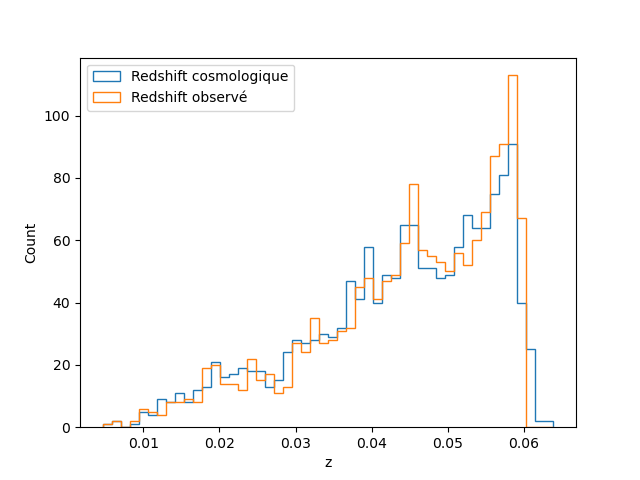
\includegraphics[width=\textwidth]{figures/redshift_draw.png}
		\caption{Distribution des redshift tirés à partir du catalogue de galaxies Uchuu. Le redshift cosmologique correspond au redshift de la position de la galaxie, le redshift observé inclue l'effet Doppler des vitesses particulières.}
		\label{fig:z_draw}
	\end{subfigure}
	\hfill
	\begin{subfigure}[c]{0.5\textwidth}
		\centering
		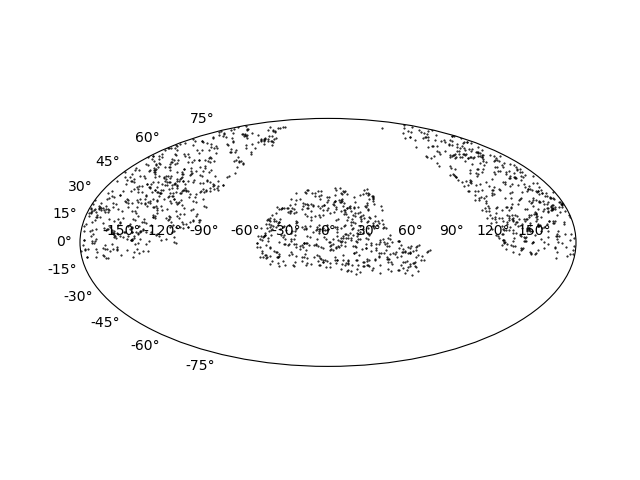
\includegraphics[width=\textwidth, trim={1cm 2.5cm 1cm 2.5cm}, clip]{figures/angular_draw.png}
		\caption{Distribution angulaire des SNe tirées à partir du catalogue de galaxies Uchuu.}
		\label{fig:ang_draw}
	\end{subfigure}
	
	\caption{Distribution spatiale des SNe tirées}
\end{figure}

De plus il est déjà possible de quantifier l'effet de la distribution intrinsèque sur la reconstruction des vitesses particulières. En effet, une erreur commise sur les modules de distances impact directement le redshift cosmologiques reconstruit, et donc les vitesses particulières (cf. Fig \ref{fig:vp_sigma_int}). Cette erreur est corrélée avec le redshift, et devient plus importante à haut redshift car $\mu(z)$ y croît plus lentement.

\begin{figure}
	\centering
	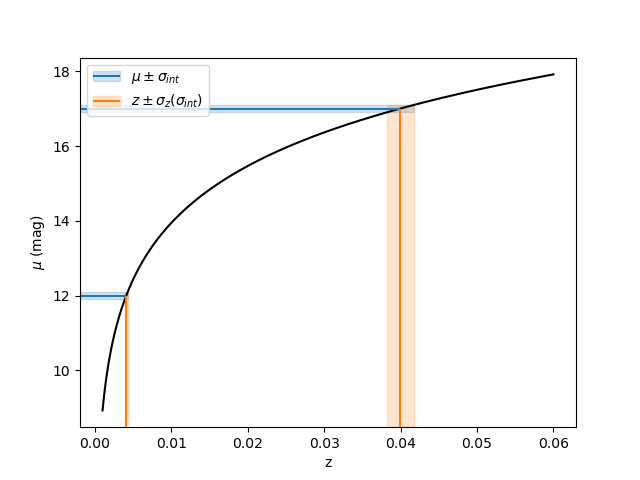
\includegraphics[width=0.8\linewidth]{figures/sigma_int_effect_vp.png}
	\caption{Illustration de l'erreur commise à $1\sigma$ sur les redshifts cosmologiques reconstruits due à la dispersion intrinsèque.}
	\label{fig:vp_sigma_int}
\end{figure}

La distribution des vitesses particulières ainsi reconstruites est représentée en Fig. \ref{fig:vp_draw}. Les vitesses particulières sont reconstruites avec une erreur moyenne de $18.4$km/s et une dispersion de $596.8$km/s. On observe bien une augmentation de l'erreur commise sur les vitesses particulières reconstruites, et cette augmentation suit l'erreur théorique due à la dispersion intrinsèque. De plus, si on calcule la moyenne des erreurs théoriques due à la dispersion intrinsèque sur l'échantillon complet, on obtient $\sigma_{v_{pec}}(\sigma_{int}) = 592.4$km/s, ce qui est proche de la dispersion observée.

\begin{figure}
	\centering
	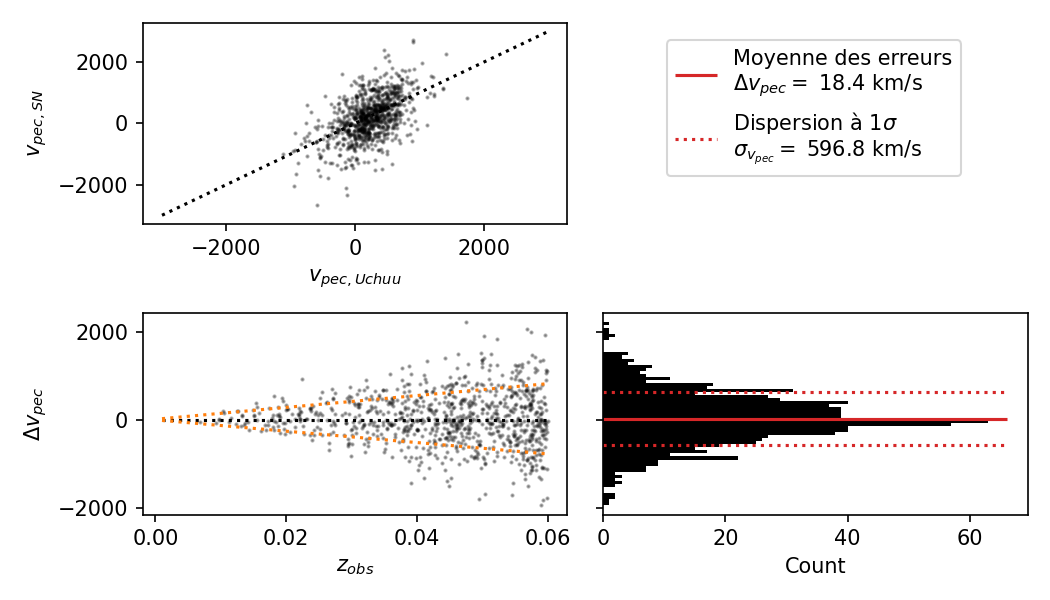
\includegraphics[width=0.9\textwidth]{figures/vp_draw.png}
	\caption{Distribution des vitesses particulières reconstruites directement à partir des SNe tirées à partir du catalogue de galaxies Uchuu. La ligne en pointillés noire (graphiques de gauche) représente la ligne de base $v_{pec, SN} = v_{pec, Uchuu}$, les lignes oranges (en bas à gauche) représente l'erreur théorique à $1\sigma$ due à la dispersion intrinsèque, et les lignes rouges pleine et en pointillés (en bas à droite) représentent respectivement la moyenne et la déviation standard des erreurs. Les barres d'erreurs en vert (en bas à gauche) montre l'évolution de la moyenne et de la dispersion des erreurs en fonction du redshift.}
	\label{fig:vp_draw}
\end{figure}

Une fois les paramètres des SNe tirés, les observations photométriques et spectroscopiques sont générées sur la base du modèle \saltd et des logs d'observation de ZTF. De telles courbes de lumière et spectres sont représentés en Figure \ref{fig:obs}.

\begin{figure}
	\centering
	\begin{subfigure}[c]{0.45\textwidth}
%		\includegraphics[width=\textwidth]{figures/lc.png}
		\caption{Courbes de lumière générées à partir des paramètres tirés. Les couleurs représentent les différents filtres utilisés.}
		\label{fig:lc}
	\end{subfigure}
	\hfill
	\begin{subfigure}[c]{0.5\textwidth}
		\centering
%		\includegraphics[width=\textwidth]{figures/spectra.png}
		\caption{Spectre généré à partir des paramètres tirés}
		\label{fig:spectra}
	\end{subfigure}
	\label{fig:obs}
	\caption{Exemple d'observations simulées pour les échantillons de SNe}
\end{figure}

\subsection{Filtrage par \pets}

Le filtrage effectué par \pets permet d'enlever les SNe qui sont mal échantillonnées. Le nombre de SNe retirées à chaque étape de sélection est indiqué en Table \ref{tab:pets}, et suivent la démarche décrite en Annexe \ref{anx:pets}.

\begin{table}
    \centering
    \begin{tabular}{p{7cm}|c|c}
         Cut & Discarded & Remaining\\
         \hline
         Total & - & 1591\\
         \saltd converge & 442 & 1149\\
         $\sigma_{t_{max}}<1$ & 31 & 1118\\
         $\chi^2(t_{max})$ est symétrique autour de $t_{max}$ & 77 & 1041\\
         Pas d'autres minimums à $8\sigma$ & 9 & 1032\\
	$|x_1|<4$ & 0 & 1032\\
	$|c|<2$ & 0  & 1032
    \end{tabular}
    \caption{SNe rejetées par \pets à chaque étape de sélection pour le lot ZTF simulé}
    \label{tab:pets}
\end{table}

 Des cas de figure typiques sont représentés en Figures \ref{fig:pets_good}, \ref{fig:pets_bad} et \ref{fig:pets_worst}.
 
La première représente le cas d'une SNe bien échantillonnée~: le minimum de la fonction $\chi^2(t_{max}$ est unique, bien défini, et présente une incertitude de $0.012$ jours, ce qui est extrêmement faible. Cette précision est telle que les intervalles à $1\sigma$ et $3\sigma$ sont indiscernables du trait plein du $t_{max}$ déterminé, qui correspond parfaitement avec celui du fit initial. Les paramètres $x_1$ et $c$ ont également des valeurs raisonnables, la SN est donc conservée.

\begin{figure}
	\begin{subfigure}{0.45\textwidth}
		\centering
		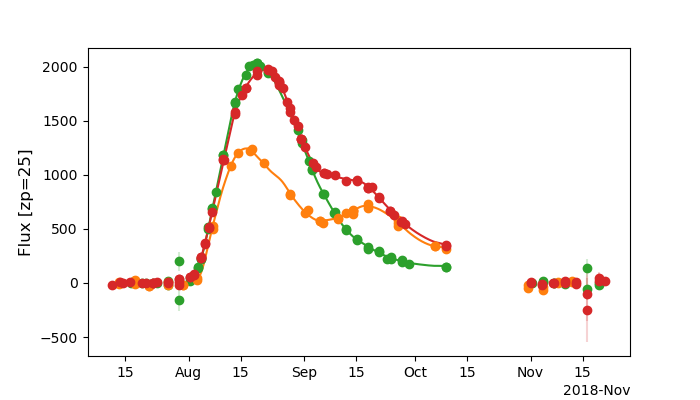
\includegraphics[width=\textwidth]{figures/276_lc_truth.png}
		\caption{Courbe de lumière simulée}
	\end{subfigure}
	\hfill
	\begin{subfigure}{0.45\textwidth}
		\centering
		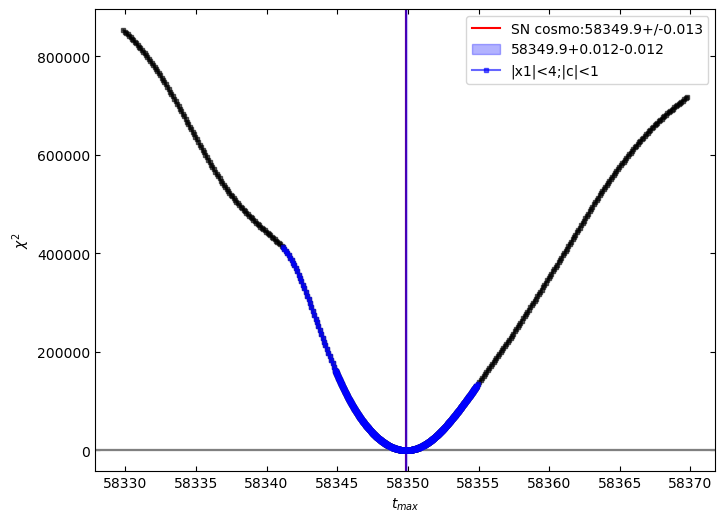
\includegraphics[width=\textwidth]{figures/276_Tmaxgrid.png}
		\caption{Évolution du $\chi^2$ avec le temps de maximum}
	\end{subfigure}
	\caption{SNe validée par \pets. Le minimum du $\chi^2$ est unique et bien défini.}
	\label{fig:pets_good}
\end{figure}
 
Le second cas de figure (Figure \ref{fig:pets_bad}), est celui d'une SNe mal échantillonnée~: le minimum de la fonction $\chi^2(t_{max}$ est toujours unique, mais mal défini car le $\chi^2$ varie peu autour du minimum, ce qui a pour conséquence une incertitude de $^{+0.764}_{-0.828}$ jours et une asymétrie du $\chi^2$. Cette aplatissement du $\chi^2$ autour du minimum a pour conséquence majeure d'entraîner de fortes variations des fonctions $x_1(t_{max})$ et $c(t_{max})$, notamment vers $t_{max}=58 810$ où les deux paramètres sortent des plages acceptables. Ce comportement est à éviter pour l'entraînement de \nacl, car l'ajustement des paramètres du modèle conjointement à ceux des SNe a plus de chance de se bloquer et d'obtenir des paramètres de standardisations anormalement élevés. Cette SN est donc rejetée.

\begin{figure}
	\begin{subfigure}{0.45\textwidth}
		\centering
		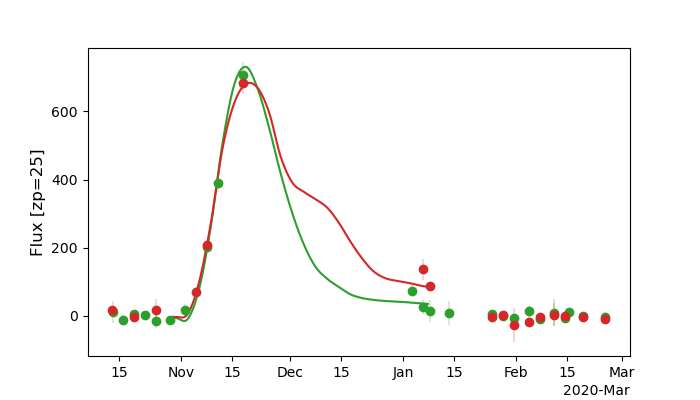
\includegraphics[width=\textwidth]{figures/10_lc_truth.png}
		\caption{Courbe de lumière simulée}
	\end{subfigure}
	\hfill
	\begin{subfigure}{0.45\textwidth}
		\centering
		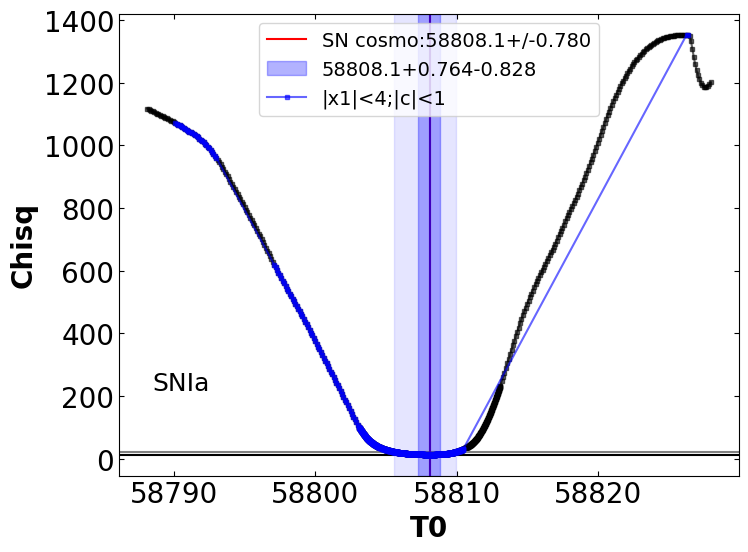
\includegraphics[width=\textwidth]{figures/10_Tmaxgrid.png}
		\caption{Évolution du $\chi^2$ avec le temps de maximum}
	\end{subfigure}
	\caption{SNe rejetée par \pets. Le minimum du $\chi^2$ est unique mais mal défini.}
	\label{fig:pets_bad}
\end{figure}

Le troisième cas de figure concerne un cas pathologique, qui a été diagnostiqué lors de ce stage et est détaillé en Section \ref{sec:min_mult}. En effet, la SNe ne présente des points de photométrie que sur la fin de sa décroissance, ce qui a pour effet de focaliser la première estimation de $t_{max}$ autour de ces points. \pets ignorant alors les minimums aux extrémités de l'intervalle de $t_{max}$ utilisés, cette SNe ne présentait qu'un minimum bien défini, avec une incertitude faible de $\pm 0.111$ jours, et était donc satisfaisante. Ce comportement a donc été modifié pour prendre en compte les minimums aux extrémités, et la détection de minimums potentiellement problématiques remontée à $\Delta \chi^2 = 64$ (équivalent à une détection à $8\sigma$) plutôt que $\Delta \chi^2 = 9$ (respectivement $3\sigma$).


\begin{figure}
	\begin{subfigure}{0.45\textwidth}
		\centering
		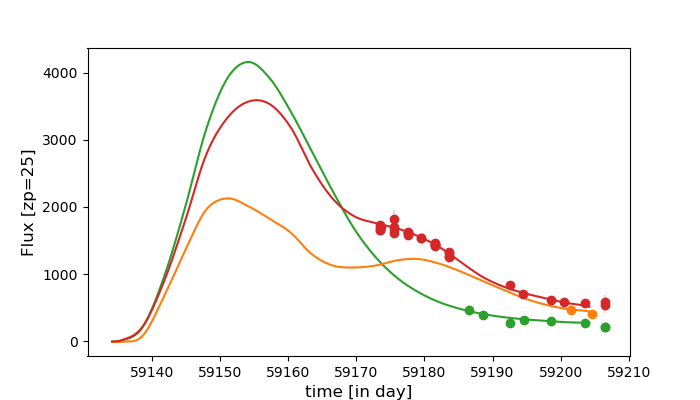
\includegraphics[width=\textwidth]{figures/544_lc_truth.png}
		\caption{Courbe de lumière simulée}
	\end{subfigure}
	\hfill
	\begin{subfigure}{0.45\textwidth}
		\centering
		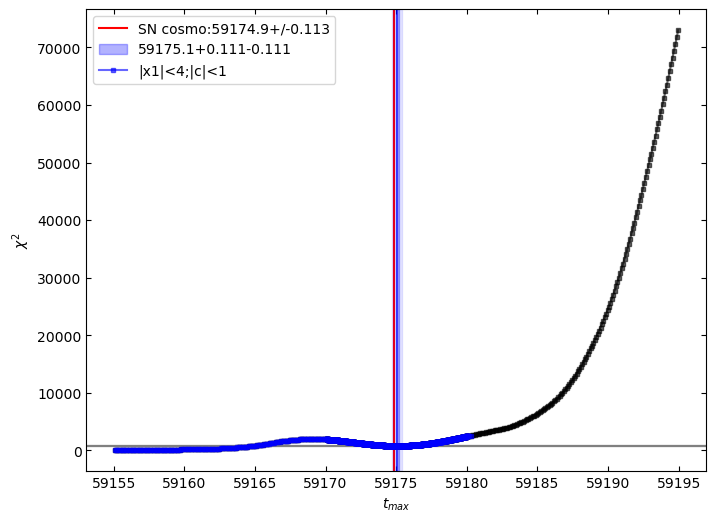
\includegraphics[width=\textwidth]{figures/544_Tmaxgrid.png}
		\caption{Évolution du $\chi^2$ avec le temps de maximum}
	\end{subfigure}
	\caption{SNe anormale validée par \pets avant correction. Le minimum du $\chi^2$ trouvé initialement est un minimum local, et l'intervalle exploré ne couvre pas la vraie valeur. }
	\label{fig:pets_worst}
\end{figure}

\subsection{Reconstruction avec \saltd}

La première reconstruction des paramètres de standardisation possible une fois les courbes de lumières simulées et traitées avec \pets est obtenue avec le modèle \saltd. Les résidus sur les paramètres reconstruits sont présentés en Figures \ref{fig:salt_residuals} et \ref{fig:salt_mu}

\begin{figure}
	\centering
	\begin{subfigure}{0.45\textwidth}
		\centering
		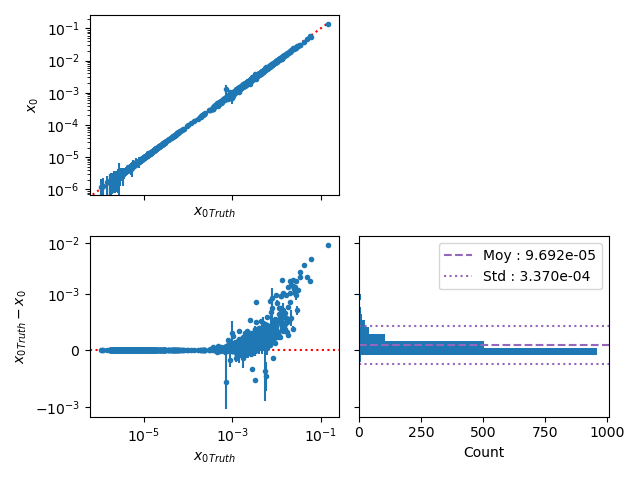
\includegraphics[width=\textwidth]{figures/salt_x0.png}
		\caption{Amplitudes, représentées en échelle logarithmique}
		\label{fig:salt_x0}
	\end{subfigure}
	\hfill
	\begin{subfigure}{0.45\textwidth}
		\centering
		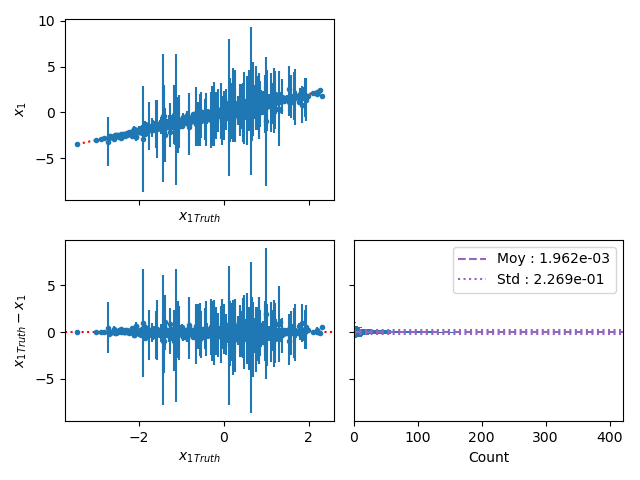
\includegraphics[width=\textwidth]{figures/salt_x1.png}
		\caption{Stretch}
		\label{fig:salt_x1}
	\end{subfigure}
	\hfill
	\begin{subfigure}{0.45\textwidth}
		\centering
		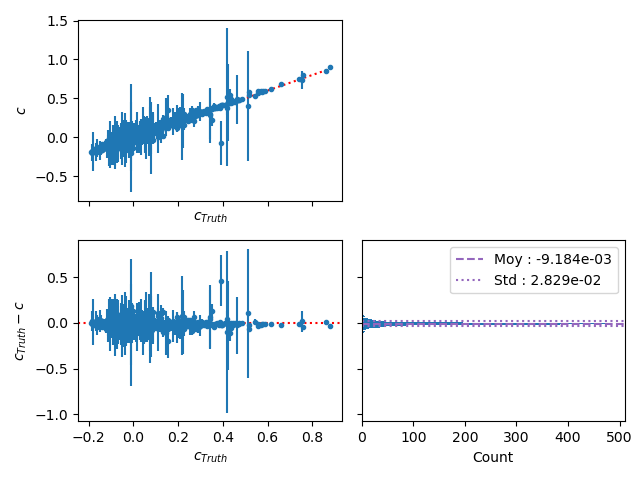
\includegraphics[width=\textwidth]{figures/salt_c.png}
		\caption{Couleurs}
		\label{fig:salt_c}
	\end{subfigure}
	\hfill
	\begin{subfigure}{0.45\textwidth}
		\centering
		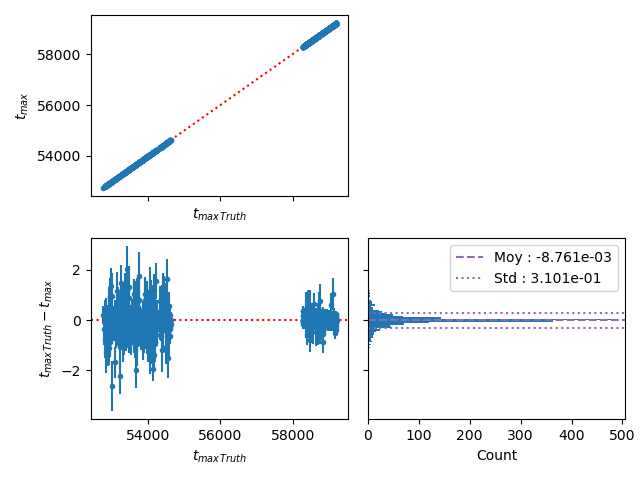
\includegraphics[width=\textwidth]{figures/salt_tmax.png}
		\caption{Temps de maximum }
		\label{fig:salt_tmax}
	\end{subfigure}
	\caption{Résidus des paramètres $(x_0, x_1, c, t_{max}$ reconstruits par \saltd}
	\label{fig:salt_residuals}
\end{figure}

Sans grande surprise, les paramètres de standardisations sont bien reconstruits puisque seules des SNe bien échantillonnées sont utilisées. On peut toutefois noter le biais qui survient pour les grandes amplitudes (cf Figure \ref{fig:salt_x0}), et les incertitudes étonnamment élevées pour certains stretch (cf Figure \ref{fig:salt_x1}) et couleurs (cf Figure \ref{fig:salt_c}), alors que les résidus des valeurs reconstruites sont faibles. Cela est du en grande partie au fait que le modèle d'erreur a été ajusté à l'aides de simulations après entraînement pour \saltd. Pour la reconstruction des temps de maximum (cf Figure \ref{fig:salt_tmax}), on peut clairement voir la distinction temporelle entre SNLS et ZTF, et il n'est pas surprenant que les résidus de SNLS soient plus importants. En effet, SNLS observe des SNe plus lointaine, donc les flux reçus sont bien plus faibles que ceux de ZTF. Cela a pour effet d'avoir des incertitudes relatives sur les flux plus importantes, et le temps de maximum est moins bien contraint.

\begin{figure}
    \centering
    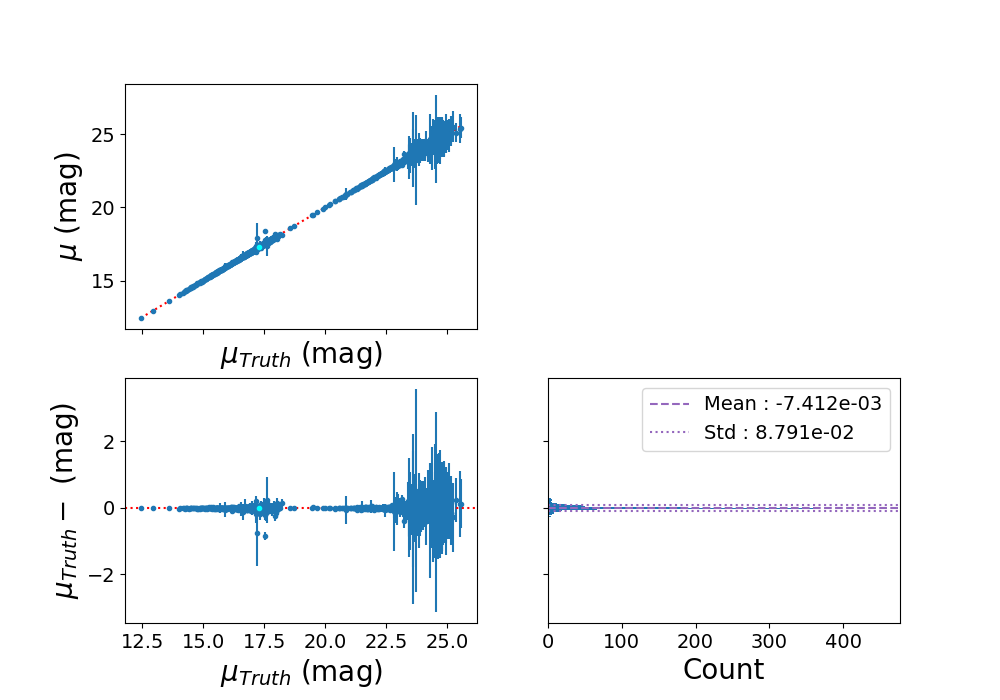
\includegraphics[width=0.8\textwidth]{figures/salt_mu.png}
    \caption{Résidus des modules de distances $\mu = -2.5\log_{10} x_0 - 0.14 \times x_1 + 3.15 \times  c$ reconstruits par \saltd.}
    \label{fig:salt_mu}
\end{figure}

Les modules de distances sont très biens reconstruits, l'erreur moyenne commise n'est que de l'ordre de $10̂{-2}$ mag. De plus comme seules les SNe de ZTF seront utilisées pour le calcul des vitesses particulières, les incertitudes élevées des SNe SNLS (moins lumineuses, donc ayant une magnitude plus élevées) ne sont pas gênantes.

\subsection{Analyse cosmologique sur les résultats \saltd}

Les vitesses particulières obtenues sont représentées en Fig. \ref{fig:vp_salt}. Les vitesses reconstruites sont en bon accord avec les vitesses injectées, mais présentent un léger biais. L'erreur moyenne n'est que de $270$km.s$^{-1}$ et l'écart type de l'erreur commise est de $791$km.s$^{-1}$, ce qui est plus élevé de 36\% que l'effet attendu de la dispersion intrinsèque, à $581$km.s$^{-1}$. On peut également noter le fait que le biais sur la moyenne des erreurs évolue avec le redshift, qui peut être à l'origine d'une part du biais non nul observé sur l'ensemble de l'échantillon, et d'autre part de l'élargissement de la dispersion. Un tel effet est intéressant puisqu'il pourrait s'agir d'un effet de flux cohérent, c'est-à-dire que les galaxies hôtes présentent toutes une même composante de vitesse par rapport à l'observateur liée à la formation d'une structure commune.

Ce biais peut également être causé par une mauvaise estimation des paramètres du modèle par \edris~: un des principal défaut des analyses cosmologiques basées sur les SNe Ia est qu'elles n'imposent pas de contraintes sur la constante de Hubble $H_0$ car elle intervient dans le calcul de la magnitude selon le modèle sous la forme d'un terme additif. Cela signifie qu'une variation du à la calibration des flux ou de la magnitude de référence en bande B $m_B$ peut être à tort interprétée comme une modification de $H_0$. Pour les vitesses particulières, un tel effet se traduirait par un déplacement vertical artificiel des modules de distance, et introduirait donc un biais sur l'ensemble des modules de distance reconstruits par \edris.

\begin{figure}
	\centering
	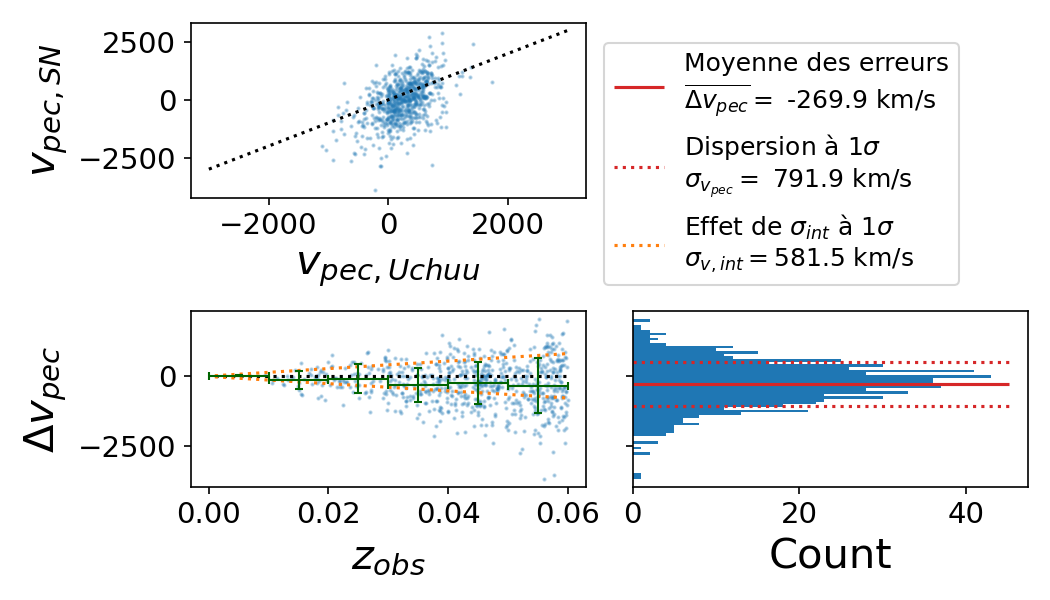
\includegraphics[width=0.8\textwidth]{figures/vp_salt.png}
	\caption{Distribution des vitesses particulières reconstruites avec \edris à partir de \saltd ($v_{pec,SN}$). La ligne en pointillés noire (graphiques de gauche) représente la ligne de base $v_{pec, SN} = v_{pec, Uchuu}$, les lignes oranges (en bas à gauche) représente l'erreur théorique à $1\sigma$ due à la dispersion intrinsèque, et les lignes rouges pleine et en pointillés (en bas à droite) représentent respectivement la moyenne et la déviation standard des erreurs. Les barres d'erreurs en vert (en bas à gauche) montre un biais de la moyenne des erreurs en fonction du redshift, il peut s'agir d'un effet de flux cohérent.}
	\label{fig:vp_salt}
\end{figure}


\subsection{Reconstruction et vitesses particulières avec \nacl}
En exécutant la même chaîne avec le résultat de \nacl, on obtient les résultats suivants.

Les résultats de l'entraînement de \nacl sont présentés en Figure \ref{fig:nacl_residuals} pour les paramètres des SNe, en Figure \ref{fig:nacl_models} pour les modèles, et en Figure \ref{fig:nacl_mu} pour les modules de distances.

\begin{figure}
	\centering
	\begin{subfigure}{0.45\textwidth}
		\centering
		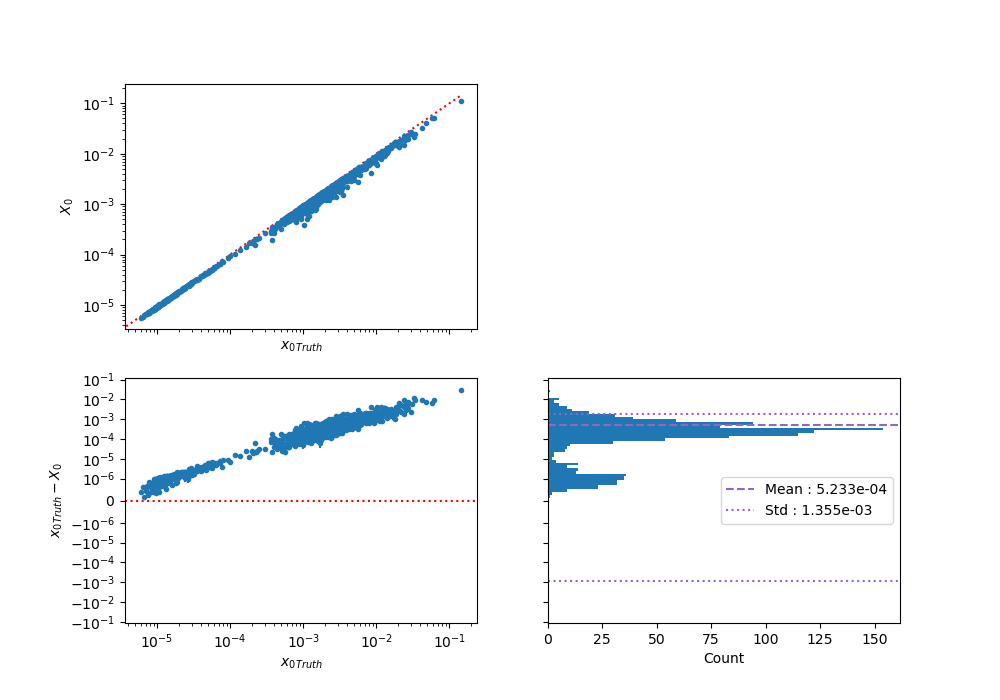
\includegraphics[width=\textwidth]{figures/nacl_x0.png}
		\caption{Amplitudes, représentées en échelle logarithmique}
		\label{fig:nacl_x0}
	\end{subfigure}
	\hfill
	\begin{subfigure}{0.45\textwidth}
		\centering
		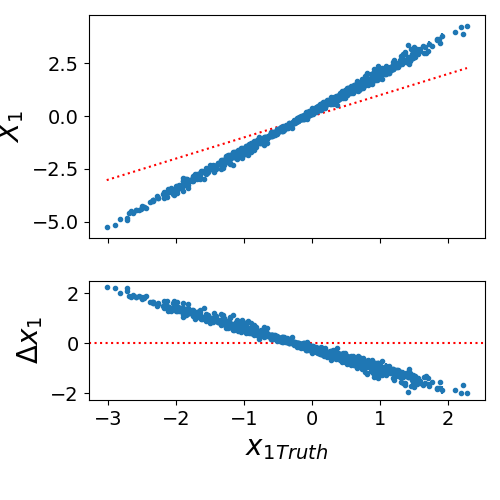
\includegraphics[width=\textwidth]{figures/nacl_x1.png}
		\caption{Stretch}
		\label{fig:nacl_x1}
	\end{subfigure}
	\hfill
	\begin{subfigure}{0.45\textwidth}
		\centering
		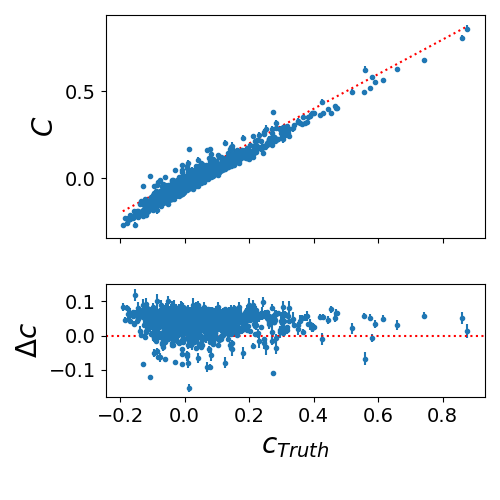
\includegraphics[width=\textwidth]{figures/nacl_c.png}
		\caption{Couleurs}
		\label{fig:nacl_c}
	\end{subfigure}
	\hfill
	\begin{subfigure}{0.45\textwidth}
		\centering
		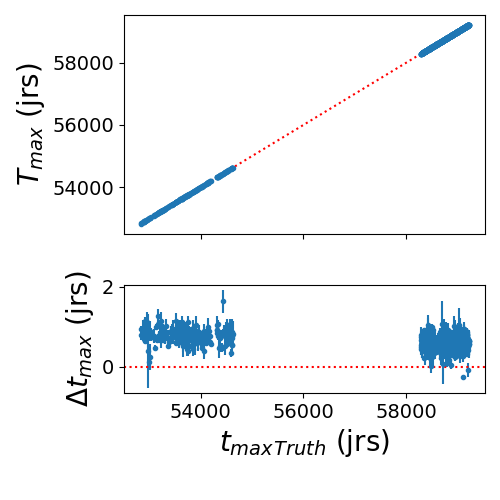
\includegraphics[width=\textwidth]{figures/nacl_tmax.png}
		\caption{Temps de maximum }
		\label{fig:nacl_tmax}
	\end{subfigure}
	\caption{Résidus des paramètres $(X_0, X_1, C, t_{max}$ reconstruits par \nacl}
	\label{fig:nacl_residuals}
\end{figure}

Les paramètres reconstruits présentent plusieurs biais, mais qui ne sont pas problématiques. En effet, le biais sur les amplitudes $X_0$ n'apparaît que pour les grandes amplitudes, qui ne concernent que les SNe à haut redshift de SNLS et dont on ne peut pas mesurer la vitesse particulière à cause de la dispersion intrinsèque. Les biais sur le stretch $X_1$ et la couleur $C$, sont principalement dus à la renormalisation des modèles $M_0^{\nacl}(p, \lambda)$ et $M_1^{\nacl}(p,\lambda)$. De même, le biais d'environ $0.6$ jours sur le temps de maximum, est causé par le ré-entraînement de $M_0^{\nacl}(p, \lambda)$.

\begin{figure}
	\centering
	\begin{subfigure}{0.45\textwidth}
		\centering
		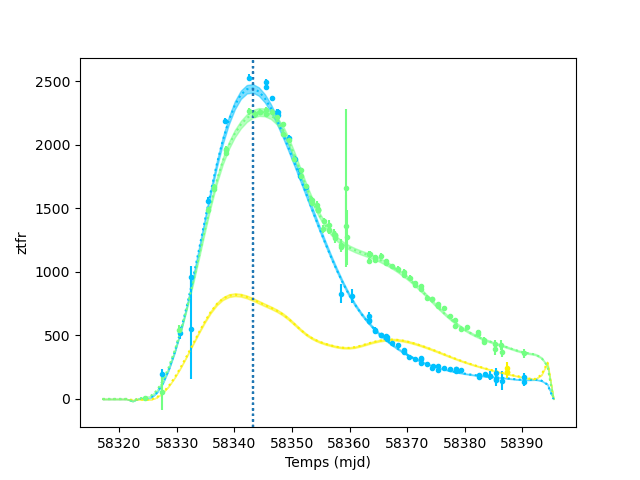
\includegraphics[width=\textwidth]{figures/nacl_lc.png}
		\caption{Courbes de lumières}
		\label{fig:nacl_lc}
	\end{subfigure}
	\hfill
	\begin{subfigure}{0.45\textwidth}
		\centering
		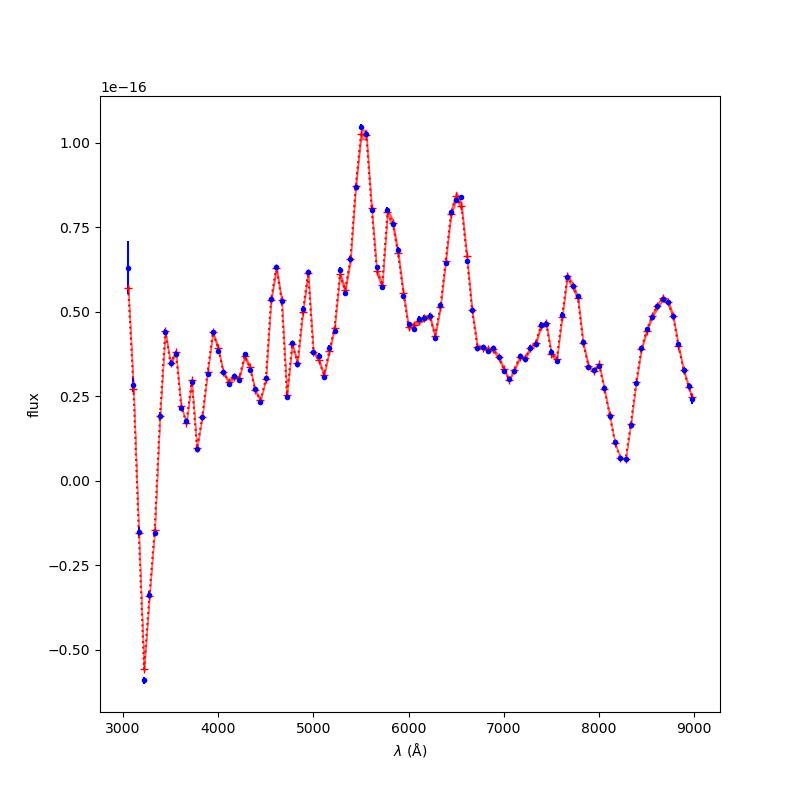
\includegraphics[width=\textwidth]{figures/nacl_spec.png}
		\caption{Spectre}
		\label{fig:nacl_sp}
	\end{subfigure}
	\caption{Exemple de courbes de lumières et de spectres avec le modèle ajusté par \nacl}
	\label{fig:nacl_lcsp}
\end{figure}

Les biais présents ne gênent en rien la modélisation des courbes de lumière ni des spectres (cf Figure \ref{fig:nacl_lcsp}) et sont purement du au ré-entraînement des modèles. Les incertitudes rapportées ne sont pas non plus aberrantes comparées à l'amplitude des paramètres.

\begin{figure}
	\centering
	\begin{subfigure}{0.9\textwidth}
		\centering
		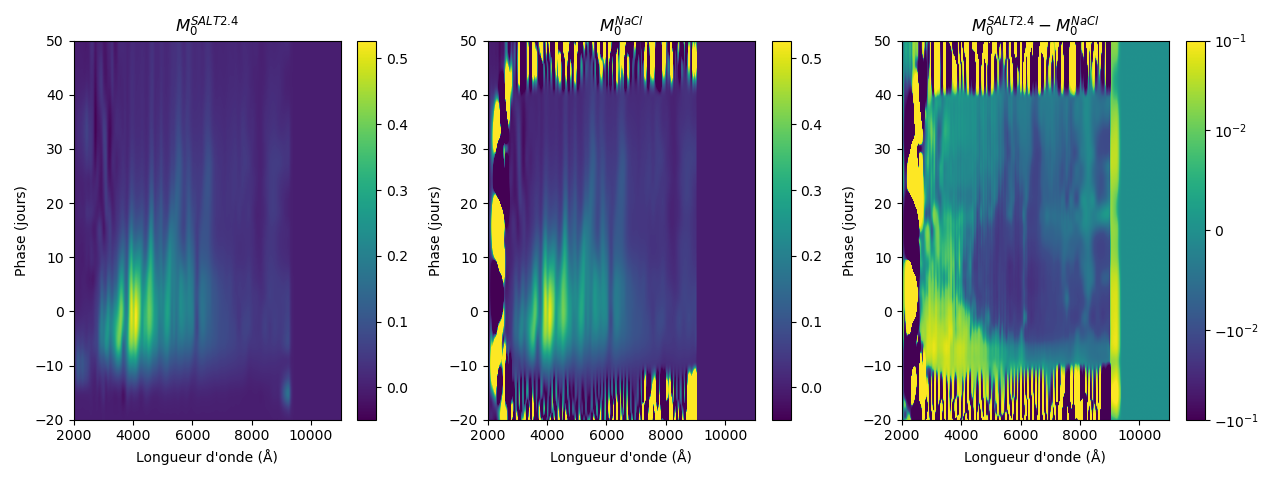
\includegraphics[width=\textwidth]{figures/nacl_m0.png}
		\caption{Modèle $M_0^{\nacl}(p, \lambda)$}
		\label{fig:nacl_m0}
	\end{subfigure}
	\hfill
	\begin{subfigure}{0.9\textwidth}
		\centering
		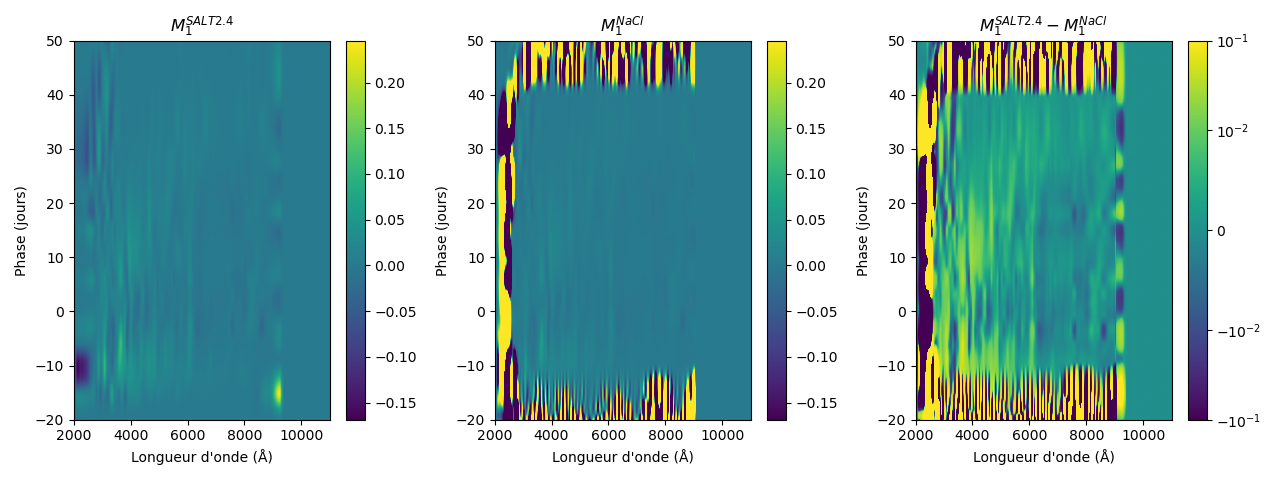
\includegraphics[width=\textwidth]{figures/nacl_m1.png}
		\caption{Modèle $M_1^{\nacl}(p, \lambda)$}
		\label{fig:nacl_m1}
	\end{subfigure}
	\hfill	
	\begin{subfigure}[c]{0.35\textwidth}
		\centering
		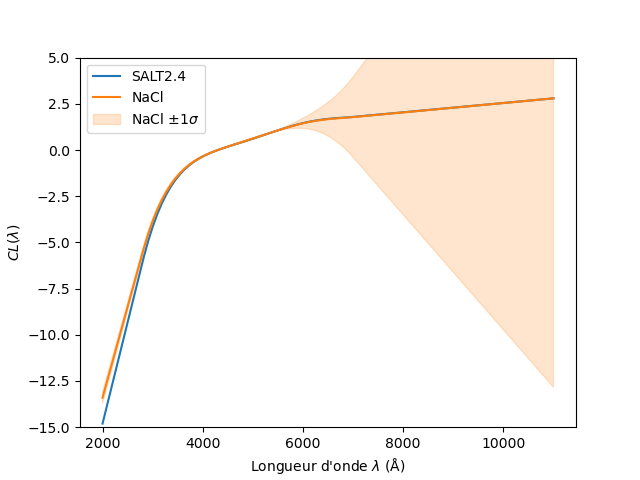
\includegraphics[width=0.8\textwidth]{figures/nacl_cl.png}
		\caption{Loi de couleur $CL(\lambda)$}
		\label{fig:nacl_cl}
	\end{subfigure}
	\hfill
	\begin{subfigure}[c]{0.6\textwidth}
		\centering
		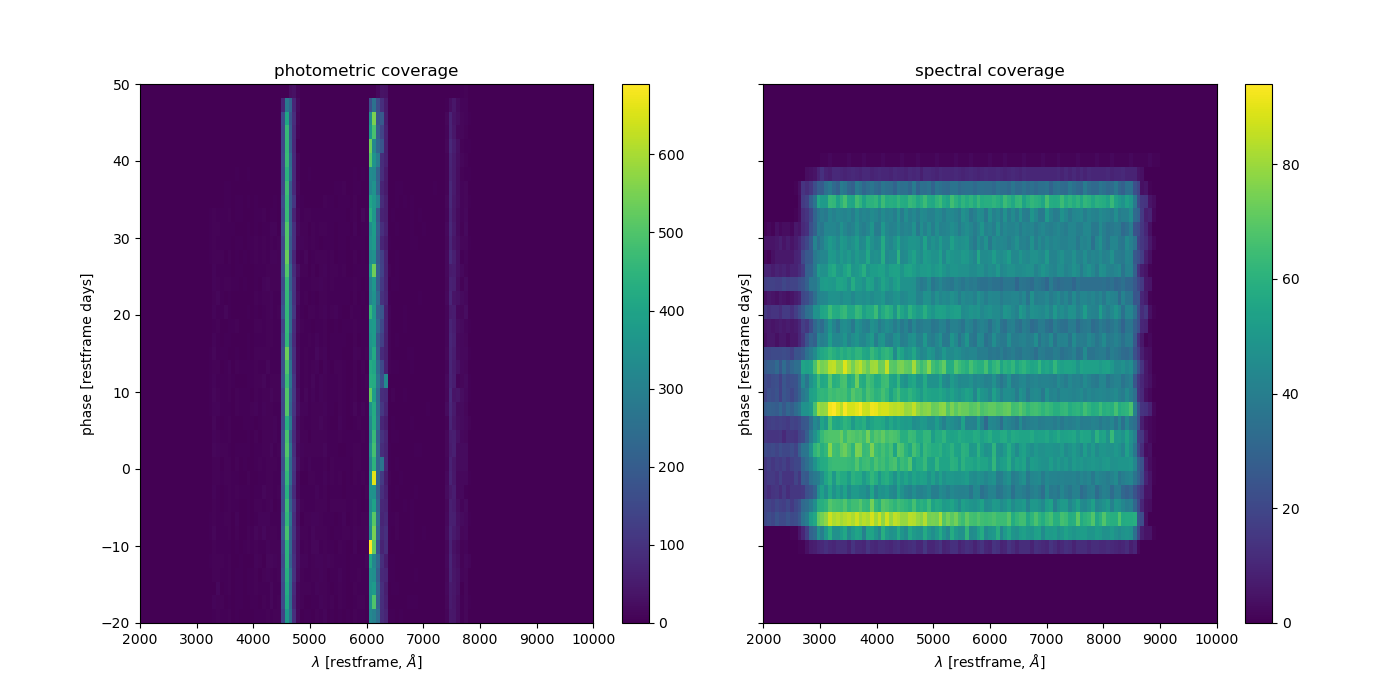
\includegraphics[width=\textwidth]{figures/nacl_coverage.png}
		\caption{Couverture du modèle par les points de photométrie (\textit{i.e.} des courbes de lumières) et les points de spectroscopie}
		\label{fig:nacl_coverage}
	\end{subfigure}

	\caption{Modèles \saltd et modèles \nacl entraînés. Les zones de fortes fluctuations des modèles entraînés, autour des bornes de la surface, est du au manque de points de données contraignant le modèle}
	\label{fig:nacl_models}
\end{figure}

Les modèles ré-entraînés semble diverger et fluctuent anormalement aux bornes de leurs ensembles de définition (cf Figure \ref{fig:nacl_m0}, \ref{fig:nacl_m1}), mais cela n'est pas un problème. En effet, ce sont des zones sur lesquels le modèle \saltd initial étaient défini, mais qui n'était pas contraintes par les données utilisées pour l'entraînement (cf. Figure \ref{fig:nacl_coverage}). Le modèle ajusté n'est donc pas fiable dans ces régions. Ces fortes fluctuations sont toutefois surprenantes, d'une part car la contrainte de régularisation (voir Annexe \ref{anx:nacl}) vise précisément à empêcher ces fluctuations, d'autre part car c'est habituellement la marque d'un sur-entraînement, pour lequel le modèle a trop de paramètres libres et manque de données pour les contraindre. En revanche, les modèles \saltd et \nacl s'accordent dans les régions contraintes par les données.

\begin{figure}
    \centering
    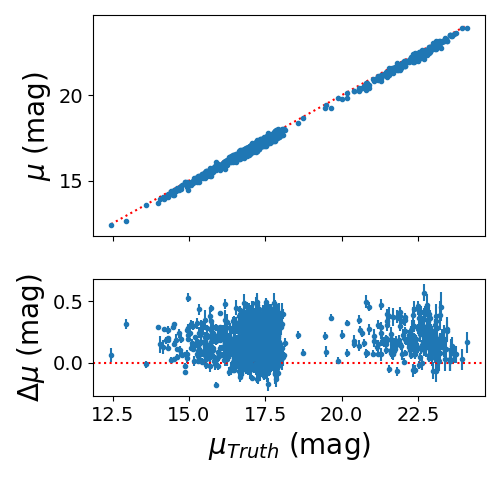
\includegraphics[width=0.8\textwidth]{figures/nacl_mu.png}
    \caption{Résidus des modules de distances $\mu = -2.5\log_{10} X_0 - 0.14 \times X_1 + 3.15 \times  C$ reconstruits par \nacl. Ils présentent un biais d'environ $-0.2$ mag, qui est causé par le ré-entraînement des modèles, mais n'est pas gênant pour l'analyse cosmologique.}
    \label{fig:nacl_mu}
\end{figure}
Les modules de distances reconstruits par \nacl présentent un biais d'environ $-0.2$ mag (cf Figure \ref{fig:nacl_mu}), mais ce biais n'est pas gênant pour la suite de l'analyse. En effet, comme mentionné précédemment, les magnitudes ne sont définies que relativement les unes aux autres.

Les vitesses particulières obtenues à l'aide d'\edris sont représentées en Fig. \ref{fig:vp_nacl}. Les vitesses reconstruites sont en bon accord avec les vitesses injectées, mais présentent un léger biais. L'erreur moyenne n'est que de $265$km.s$^{-1}$ et l'écart type de l'erreur commise est de $686$km.s$^{-1}$, ce qui correspond à une augmentation de la dispersion de 18\% par rapport à l'effet attendu de la dispersion intrinsèque.

\begin{figure}
	\centering
	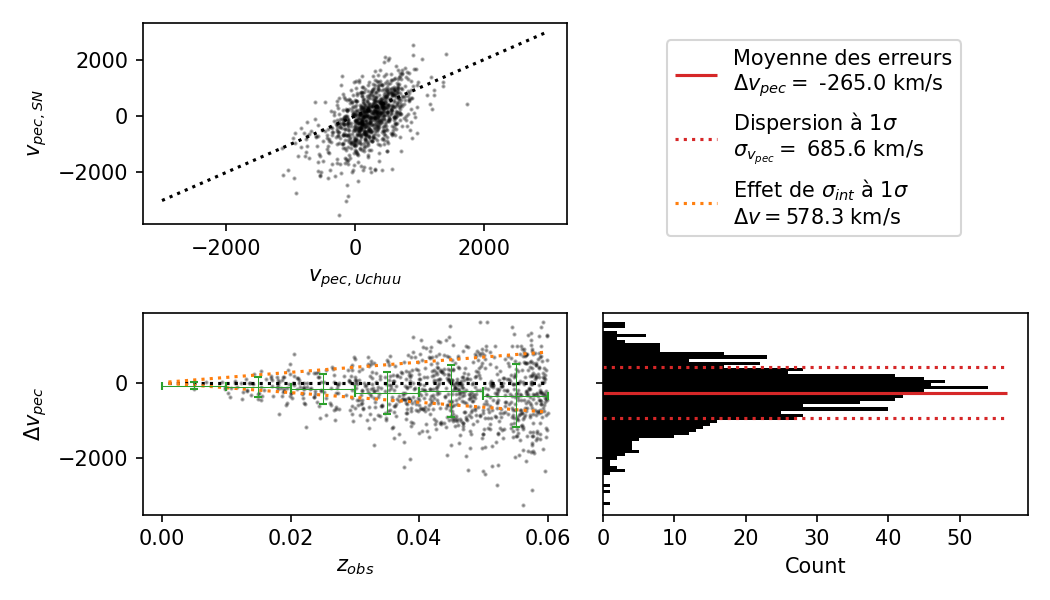
\includegraphics[width=0.8\textwidth]{figures/vp_nacl.png}
	\caption{Distribution des vitesses particulières reconstruites avec \edris à partir de \saltd ($v_{pec,SN}$). La ligne en pointillés noire (graphiques de gauche) représente la ligne de base $v_{pec, SN} = v_{pec, Uchuu}$, les lignes oranges (en bas à gauche) représente l'erreur théorique à $1\sigma$ due à la dispersion intrinsèque, et les lignes rouges pleine et en pointillés (en bas à droite) représentent respectivement la moyenne et la déviation standard des erreurs. Les barres d'erreurs en vert (en bas à gauche) montre un biais de la moyenne des erreurs en fonction du redshift, il peut s'agir d'un effet de sélection ou d'un flux cohérent.}
	\label{fig:vp_nacl}
\end{figure}

Le biais entre les vitesses reconstruites par \saltd et \nacl étant semblables, son origine ne provient pas de l'algorithme utilisé pour la reconstruction des paramètres de standardisation. En revanche le ré-entraînement du modèle pour \nacl a permis une meilleure estimation des vitesses particulières, puisque la dispersion additionnelle sur l'effet de la dispersion intrinsèque a été réduit de 38\% à 18\%.


\section{Problèmes identifiés dans le pipeline \lemaitre et corrections apportées}

J'ai identifié et traité différents problèmes et erreurs au sein du pipeline \lemaitre. Certains étaient triviaux à traiter une fois identifiés, tel que des erreurs dues à des différences d'encodage (sur 32 ou 64 bits) de certaines valeurs lors de sauvegardes et chargements de données entre des modules, d'autres plus compliqués, et quelques uns restent encore non résolus. Les problèmes rencontrés peuvent être regroupés en deux catégories~: ceux causés par l'utilisation de mauvaises valeurs de méta-paramètres, qui ne remettent pas en cause les méthodes mais nécessitent un ajustement de ces paramètres, et ceux liés directement aux méthodes utilisées.

\subsection{Problèmes liés à des valeurs de méta-paramètres}

\subsubsection{Minimums multiples dans \pets}
\label{sec:min_mult}

Un premier problème est apparu lors de l'utilisation de \pets concerne la caractérisation des SNe pour l'entraînement de \nacl. Certaines SNe ne présentent des points de mesure que sur la croissance ou la fin de la décroissance de leur luminosité pour des raisons observationnelles tel que leur concordance avec le début ou la fin d'une période d'observation. Ces SNe posent alors le problème d'être difficiles à caractériser, bien que parfaitement décrites par \saltd. En particulier, les SNe qui n'ont des points de photométrie que sur la fin de leur décroissance présentent souvent deux minimums locaux (voir Figure \ref{fig:pets_worst}). Comme \pets utilise le point de données de flux le plus élevé comme point de départ pour ajuster le $t_{max, 0}$ à partir duquel la grille est générée, il peut converger vers un minimum local bien marqué et générer une grille ne couvrant pas le minimum global au vrai temps de maximum.

La solution employée ici a été de remonter la détection des autres minimums de $3\sigma$ à $8\sigma$, et de retirer les SNe ainsi identifiées comme problématiques du lot de données à analyser. Une meilleure solution, implémentée pour les utilisations futures de \pets, est d'augmenter l'intervalle couvert par la grille, mais cela nécessite en contrepartie soit de diminuer sa résolution et donc l'estimation des incertitudes, soit d'utiliser plus de points, ce qui augmente le temps de calcul. A noter que si ces SNe sont bien décrites par \saltd, elles ne sont pas intéressantes pour entraîner \nacl puisqu'elles ne comportent que peu de point de données et ne couvrent qu'une faible fraction des phases. Elles pourraient être fittées après entraînement afin de gagner en statistiques, mais le gain restera minime puisqu'elles demeurent assez rares (environ ~1\% des SNe respectant par ailleurs les autres critères de \pets).

De plus c'est un problème qui est particulièrement présent dans mes simulations, mais devrait être rare lors de l'utilisation de données réelles. En effet, puisque seules des SNe Ia sont générées, elles sont reconstruites en partant du principe que ce sont des SNe Ia. Sur des données réelles, rien ne garantit qu'un événement transitoire dont on a observé uniquement la décroissance soit une SNe Ia. Il pourrait s'agir d'une SNe Ib, Ic, II, ou d'un autre type d'événement cataclysmique. Dans ce cas, l'événement ne sera pas classé avec certitude comme SN Ia, et ne passera pas donc par \pets.
 

\subsubsection{Domaine de définition des modèles}

Un deuxième problème qui est survenu vient du domaine de définition des modèles dans \nacl. Initialement, les modèles couvraient l'intervalle $[-20; 50]$ en phase et $[2000; 9000]$ Ångströms en longueur d'onde. Or, pour le calcul des flux des points de photométrie, il arrive que le support de la transmission du filtre sorte du domaine de définition en longueur d'onde des modèles. Cela revient à couper les filtres et fausse le flux calculé, ce qui en retour biaise la reconstruction des paramètres de standardisation puisque le modèle s'adapte pour compenser cette coupure.

La solution a été simplement d'augmenter le domaine de définition des modèles, de 2 000 à 11 000 Ångströms. Aux redshifts considérés, les filtres ne sortent plus du modèle et l'évaluation redevient correcte.

\subsubsection{Régularisation et contraintes dans \nacl}

Un autre problème identifié dans \nacl concerne les coefficients de régularisation $\mu_{reg}$ et de contraintes $\mu_{cons}$. Les premiers tests effectués utilisaient $\mu_{reg} = 1$ et $\mu_{cons} = 10^{-10}$, mais ces valeurs étaient trop faibles et ne permettaient pas d'imposer aux modèles les contraintes et la régularisation voulus. Une des conséquences majeures étaient une mauvaise convergence, et une surestimation des incertitudes sur les paramètres reconstruits.
Il s'est avéré que prendre des valeurs $\mu_{reg} = 100$ et $\mu_{cons} = 10^6$ donnent une bien meilleure convergence, et ne surestiment plus les incertitudes.

\subsubsection{Quality cuts pour \edris}
\label{sec:qc_edris}
Dès les premières tentatives de production de diagrammes de Hubble à partir de la reconstruction avec \saltd, la convergence d'\edris est apparue comme très dépendante des données. En particulier, la présence d'outliers est susceptibles de coincer le fit des paramètres et de la cosmologie. Les outliers peuvent apparaître soit lors de la génération (\textit{i.e.} les paramètres sont extrêmes mais probables au vu des distribution), soit lors de la reconstruction (\textit{i.e.} la SNe n'était pas aberrante, mais elle est mal reconstruite). L'amplitude des coefficients de la matrice de covariance des paramètres $(x_0, x_1, c)$ a un impact particulièrement important sur la convergence. C'est l'une des raisons qui a motivée l'exploration et la résolution du problème précédent~; une mauvaise convergence de \nacl donnait un point de départ aberrant pour la matrice de covariance pour \edris.

Cela a aussi conduit à appliquer des quality cuts semblables à ceux d'Union 3 aux paramètres reconstruits afin de retirer d'éventuels outliers ou SNe mal reconstruites.

\subsection{Problèmes liés aux méthodes}

\subsubsection{Effets d'une mauvaise convergence }

J'ai évoqué comme conséquences des problèmes précédents une mauvaise convergence des modules \nacl ou \edris. Dans les faits, cette mauvaise convergence est caractérisée par plusieurs symptômes, le plus problématique concernant la hessienne du problème $\mcl H$.

Comme il serait trop coûteux d'estimer les incertitudes tout au long de l'optimisation, la solution retenue pour le pipeline \lemaitre est d'utiliser la borne de Cramer-Rao comme estimateur de la covariance. À un coefficient multiplicatif près dépendant de la formulation exacte du problème, la covariance est obtenue en inversant la matrice d'information de Fisher, qui est ici égale la hessienne 
\begin{equation}
	Cov = \mcl I^{-1} = \mcl H^{-1}
\end{equation}
et les incertitudes sont directement obtenues en prenant les racines carrées des coefficients diagonaux
\begin{equation}
	\sigma_i = \sqrt{Cov_{ii}} = \sqrt{(\mcl H^{-1})_{ii}}
\end{equation}

Le problème qui survient alors est qu'en cas d'absence de convergence ou de mauvaise convergence, la hessienne peut ne pas être définie positive, ce qui rend les incertitudes indéterminées. Ce problème est survenu à de nombreuses reprises, bien souvent du à un mauvais point de départ ou des outliers.

Dans le cas de \nacl, cela a mis en lumière la nécessité d'avoir une bonne convergence dans la première estimation des paramètres des SNe. En cas de mauvaise estimation, le modèle essaie de surcompenser cette mauvaise estimation pour décrire les données lors du dernier fit. Comme il n'arrive pas à converger correctement, il se bloque généralement dans une région de l'espace des paramètres où la hessienne n'est pas définie positive, ce qui a permis d'identifier ce type de problèmes.

\subsubsection{Dégénérescence entre $\beta$ et $\sigma_{int}$} 

Il existe une dégénérescence entre le coefficient $\beta$ de la formule de Tripp et le paramètre de dispersion intrinsèque $\sigma_{int}$ dans \edris, biais qui est particulièrement marqué lorsque l'incertitude sur la couleur $\sigma_c$ est élevée. Ce problème était déjà connu, mais a été confirmé sur les simulations produites lors de ce stage lorsque la reconstruction est effectuée avec \saltd. Ce n'est pas le cas pour la reconstruction avec \nacl car les erreurs sont sous-estimées pour une raison encore inconnue, mais ce problème pourrait également survenir à l'avenir. La solution retenue est alors de fixer la dispersion intrinsèque à sa valeur utilisée pour les simulations, $\sigma_{int} = 0.1$, puisqu'il s'agit de la dispersion observée expérimentalement.

\subsubsection{Condition d'arrêt du gradient conjugué dans \edris}

Lors de l'utilisation d'\edris, j'ai été amené à me documenter sur le détail de la méthode utilisée. En particulier, l'optimisation utilisée est décrite dans \cite{martens_deep_2010}, et mentionne explicitement que pour un problème linéaire $Ax = b$, les méthodes de gradient conjugué ne minimisent pas l'erreur quadratique $\norm{Ax-b}^2$ mais la forme quadratique $\phi(x) = \frac{1}{2} x^T A x - b^T x$. Bien que ces deux formulations présentent le même minimum global, une solution acceptable mais sous-optimale pour l'un peut s'avérer être mauvaise pour l'autre. En particulier lors d'une exécution de gradient conjugué, si $\phi(x)$ est bien décroissante, $\norm{Ax-b}^2$ fluctue violemment et ne commence à tendre vers 0 qu'à la fin de l'optimisation. Pourtant, les conditions d'arrêt des implémentations de gradient conjugué se basent souvent sur $\norm{Ax-b}^2$ et non $\phi(x)$, potentiellement car cette dernière n'est pas bornée par 0. L'auteur propose alors de modifier la condition d'arrêt pour la conditionner au taux de réduction de $\phi$, moyenné sur $k$ itérations
\begin{equation}
	i > k \qq{et} \phi(x_i) < 0 \qq{et} \frac{\phi(x_i) - \phi(x_{i-k})}{\phi(x_i)} < k \epsilon
\end{equation}

Le problème pour \edris  vient alors de son implémentation. Afin d'accélérer l'évaluation des log-vraisemblance et de leurs dérivées, \edris a été intégralement implémenté en \texttt{JAX}\footnote{\href{https://jax.readthedocs.io/en/latest/}{https://jax.readthedocs.io/en/latest/}}. Ce package propose une ré-implémentation des packages \texttt{python} usuels pour qu'ils soient compatibles avec l'optimisation proposée par \texttt{JAX}, en particulier le package \texttt{scipy} et son implémentation du gradient conjugué. Cependant, son implémentation initiale et la ré-implémentation en \texttt{JAX} utilisent toutes les deux la conditions d'arrêt déconseillée par \cite{martens_deep_2010}, ce qui peut avoir un impact non négligeable sur la convergence d'\edris.

Ce problème demeure à ce jour non résolu d'une part car son effet, s'il est bien présent, n'était pas la cause majeure d'une mauvaise convergence (voir notamment \ref{sec:qc_edris}), et d'autre part car sa résolution est compliquée puisqu'elle nécessite d'ajouter une condition d'arrêt non déterministe à la fonction de gradient conjugué, ce dont \texttt{JAX} ne s’accommode pas trivialement.


\chapter{Travail futur}
\consignes{prolongements possibles du travail de stage : exposé de ce qu’il reste éventuellement à faire pour que les résultats soient complètement obtenus, et de la façon dont le travail pourra être poursuivi par l’entreprise dans le futur}

\section{Finalisation du travail effectué lors du stage}

Comme évoqué en Section \ref{sec:res_fs8}, l'analyse $f\sigma_8$ n'a pas encore pu être réalisée, et constituera une partie de mon travail sur les prochains mois, en parallèle du début de ma thèse. Une première estimation est prévue à l'aide d'une approximation du champ de densité de la simulation Uchuu reposant sur la méthode décrite dans \cite{carrick_cosmological_2015} afin de tester et me familiariser avec la méthode de comparaison densité-vélocité pour estimer $f\sigma_8$. L'objectif est d'ensuite refaire cette analyse en utilisant cette fois un champ de densité inféré par BORG, afin d'en avoir une meilleure reconstruction.
 
\section{Postérité pour l'entreprise}

Mes deux contributions majeures aux modules et outils existants sont d'une part la génération des SNe suivant un catalogue de galaxies, et l'intégration des modules du pipeline \lemaitre. Les simulations que j'ai produites sont actuellement utilisées par d'autres doctorants afin de tester individuellement les modules \nacl et \edris.

La génération des SNe est effectuée à l'aide du module \skysurvey, mais il s'agit d'une nouvelle fonctionnalité qui n'était pas disponible auparavant. Si le tirage utilise actuellement les positions des SNe suivant le catalogue Uchuu BGS, il est possible d'utiliser n'importe quelle autre catalogue de galaxies ou plus généralement n'importe quelle table de coordonnées $(RA,DEC,Z)$. Mon implémentation est actuellement en cours d'intégration au module \skysurvey comme méthode potentielle de tirage des positions, afin de pouvoir être réutilisée pour des analyses futures.

L'intégration des modules du pipeline \lemaitre a eu lieu progressivement tout au long de mon stage, sous le nom du module \textsc{george}. Il réutilise le code que j'ai développé afin de faire communiquer les différents modules, et permet également une gestion des versions des modules ainsi que le lancement d'une analyse complète lorsqu'un des modules est mis à jour.


\chapter{Bilan personnel}
\consignes{bilan des principaux apprentissages professionnels et leur mise en perspective pour le futur professionnel}

Au cours de ce stage, j'ai été amené à réaliser un travail de recherche à plein temps au sein d'une équipe. Cette expérience était plutôt nouvelle, car si j'avais déjà effectué un stage de recherche au cours de ma césure à l'Oskar Klein Center, à Stockholm, j'avais moins de contacts et contraintes avec une équipe travaillant sur un sujet commun. Il s'agissait d'estimer le gain sur la localisation de sources d'ondes gravitationnelles à l'aide du champ de densité des galaxies, et constituait également une analyse impliquant plusieurs traceurs. J'ai du pour cela utiliser des packages python déjà développés tels que \textsc{bilby}\footnote{\href{https://lscsoft.docs.ligo.org/bilby/index.html}{https://lscsoft.docs.ligo.org/bilby/index.htm}} et les modifier pour mon utilisation, mais mes développements étaient assez distants des équipes de recherches à l'origine de ces packages. Lors du présent stage, j'ai était en revanche complètement impliqué dans le développement du pipeline \lemaitre. Mes tâches m'ont amené à discuter avec les chercheurs et doctorants travaillant sur toutes les étapes de l'analyse cosmologique, et à devoir comprendre le fonctionnement de chaque modules pour les utiliser correctement. Cette dynamique était donc très différente de celle de mon stage de césure.

Ce stage a également été ma première occasion d'assister à une conférence, puisque j'ai eu la chance d'assister au meeting DESI 2024 qui a eu lieu début juillet à Marseille. Cette expérience a été très enrichissante car j'ai pu discuter avec des chercheurs du monde entier travaillant sur des problématiques diverses liées aux données DESI, et découvrir leurs travaux. Cela m'a aussi permis de rencontrer physiquement certains chercheurs qui travaillait également sur les analyses jointes entre DESI et ZTF, et avec qui j'avais pu échanger par messages. Lors de ce meeting, j'ai également pu présenter mon travail lors des sessions \textit{Spotlight Talks}, qui consistaient en une rapide succession de présentations par des doctorants, stagiaires ou post-doctorants, d'une minute chacune avec une unique slide comme support visuelle. Cet exercice étaient particulièrement instructif puisqu'il a nécessité de sélectionner les informations clés de mon travail et de les synthétiser.

Je me sens bien plus confiant pour débuter ma thèse à l'issu de ce stage qu'avant. Je pense qu'il m'a permis de développer des compétences de communication et d'échange au sein d'une équipe comme des techniques de programmation et d'analyse, ce qui est essentiel à tout travail de recherche moderne.


\chapter{Enjeux éthiques}
\consignes{prise de recul sur les enjeux d’ordre éthique}

\section{Éthique de la recherche}

La recherche contient nécessairement une dimension éthique dans la manière de la mener. Un chercheur doit faire preuve d'intégrité et d'honnêteté intellectuelle, même si ses résultats vont à l'encontre de ses croyances. Cette dimension a pleinement été prise en compte lors de mon stage puisque ma tâche principale était justement de faire remonter les problèmes rencontrés dans le pipeline \lemaitre, et de m'assurer que tout comportement étaient soit compris, soit explicable par un effet précis, auquel cas l'effet doit être quantifié.

Il est également important de mentionner une pratique devenue courante, le \textit{blinding} des données. Cela consiste en une altération volontaire des données avant réalisation de l'analyse, afin de s'assurer que l'analyse n'est pas biaisée par un a priori sur ces données ou le modèle choisi pour les décrire. Un bon modèle de \textit{blinding} doit respecter plusieurs critères~: la qualité des données et leurs propriétés statistiques doit être conservée, il doit être difficile de l'inverser -- pour éviter que les données réelles puissent être extraites et utilisées telles quelles -- et il doit viser des paramètres précis, sans affecter les variables et diagnostiques de l'analyse. Dans le cas de DESI (\cite{andrade_validating_2024}), le \textit{blinding} est effectué en décalant les redshifts à l'aide d'une cosmologie et d'un facteur de croissance des structures fixés et inconnus des chercheurs chargés de l'analyse. La méthode du \textit{blinding} du lot de donné réel utilisé par le pipeline \lemaitre n'a pas encore été communiquée, mais intervient sur les flux mesurés pour les décaler.

\section{Égalité des genres}

Concernant l'égalité des genres, il existe toujours au sein de la recherche une grosse disparité dans les proportions d'hommes et de femmes, en partie due aux proportions déjà inégales en universités et écoles d'ingénieures. Il est également intéressant de noter la sur-représentation des femmes aux postes administratifs et de gestion. Je n'ai pas noté de discriminations lors de mon stage, en revanche j'ai parfois entendu des propos déplacés ou sexistes venant de chercheurs plus âgés dans des contextes informels. Ces comportements relèvent du sexisme ordinaire et demeurent problématiques, mais ne donnent pas lieu à une différence de traitement entre hommes et femmes pour l'accès aux postes, la parole lors des réunions ou des présentations, ou encore l'attribution du premier auteur lors de la publication des papiers.

Sorbonne Université a mis en place une cellule d'écoute et d'aide pour lutter contre les VSS, et j'ai pu voir des affiches se sensibilisations sur les comportements sexistes dans les bâtiments pour alerter sur ces questions.

\section{Impact environnemental}

L'impact environnemental de la recherche fondamental est non négligeable. Si on peut pointer du doigt les accélérateurs, télescopes et supercalculateurs nécessaires à l'avancée de la science, il ne s'agit pas du point le plus critique pour la réduction des émissions de gaz à effet de serre et de consommation d'énergie. En effet, lors du meeting DESI 2024, une présentation lors d'une session plénière a été consacrée à l'étude de l'impact environnemental de la collaboration. Et loin devant l'utilisation du NERSC pour les simulations et analyses, l'activité la plus polluante était les meetings internationaux eux-mêmes puisqu'ils engendraient de nombreux déplacements, généralement en avion. Cela engendre également un coût que tous les chercheurs ne peuvent pas couvrir, et contraint fortement les emplois du temps.

Ces problèmes n'ont pas encore résolu à une échelle globale mais des solutions commencent à être proposés. Par exemple le \textit{International Centre for Radio Astronomy Research} a organisé le \textit{2024 Astronomical Society of Australia Annual Scientific Meeting} selon une politique \textit{online-first}, sur la base de l'article \cite{sarabipour_changing_2021}. Cela signifie que le principal canal de communication n'est pas le présentiel, mais en ligne. Les présentations sont également retransmises, et les chercheurs sont invités à participer à des \textit{local Hub Day}, des rencontres entre scientifiques d'une même région ne nécessitant que peu de transports. Cela réduit donc les émissions polluantes d'une part, les coûts d'autre part, et permet également une meilleure inclusion des personnes handicapées ou ne pouvant se déplacer internationalement pour diverses raisons. Cette initiative est particulièrement intéressante, puisqu'elle essaye de concilier les besoins des rencontres internationales de chercheurs aux problèmes environnementaux et sociaux à l'aide des outils en ligne perfectionnés pendant la pandémie de COVID-19.



\appendix
\chapter{Annexes}
\pagenumbering{roman}

\section{Fonctionnement des modules}

\subsection{\pets}
\label{anx:pets}

PETS a pour but de sélectionner les SN qui sont suffisamment bien échantillonnées pour l'entraînement du modèle par NaCl.
Le fonctionnement de PETS est découpé en 3 étapes, tous utilisant le modèle \saltd déjà entraîné~:
\begin{enumerate}
\item Une sélection des points de données utilisables.
\item La réalisation d'une grille de temps de maximums et des fits associés à chacun de ces temps
\item La sélection des SNe
\end{enumerate}

La sélection des points de données est effectuée en rejetant itérativement les points de données à plus de 3$\sigma$ du fit \saltd. Ensuite, en partant du $t_{max, 0}$ d'un fit complet des points restants, une grille de temps de maximum est réalisé. Elle contient 150 points dans les intervalles $[t_{max, 0} - 20 ; t_{max, 0} - 5]$ et $[t_{max, 0} +5; t_{max, 0} + 20]$ et 1000 points dans l'intervalle $[t_{max, 0} - 5 ; t_{max, 0} + 5]$. Le modèle est alors fitté sur les données en fixant le temps de maximum à un de ces points, puis PETS analyse la courbe $\chi^2(t_{max})$ afin de garder ou rejeter la SN. Une SN est gardée si~:
\begin{enumerate}
\item $\chi^2(t_{max})$ présente un minimum global à $t_{min}$, qui n'est pas aux bords de l'intervalle $[t_{max,0} - 20 ; t_{max, 0} + 20]$
\item L'incertitude sur $t_{min}$ est inférieure à 1 jour.
\item L'écart entre les incertitudes positives et négatives à 3$\sigma$ est inferieur à $0.3$, ce qui caractérise la symétrie de $\chi^2(t_{max})$ autour de $t_{min}$.
\item $\chi^2(t_{max})$ ne présente pas d'autres minimums à 8$\sigma$ de ce minimum global, \textit{i.e.} il n'y a pas d'autres minimums proches susceptibles de coincer le fit de NaCl.
\item Les valeurs de $x_1$ et $c$ fittées sont respectivement inférieures à 4 et 2, ce qui impose que le fit ne décrit pas une SN extrêmement distordue (bien qu'elle soit toujours décrite par le modèle).
\end{enumerate}

Une version mise à jour de PETS utilisant un modèle NaCl pré-entraîné à la place de \saltd est en cours de développement, mais je ne l'ai pas utilisée.


\subsection{\nacl}
\label{anx:nacl}

\subsubsection{Modélisation des SNe}

\nacl consiste en une implémentation d'un modèle type \texttt{SALT}, avec quelques améliorations. Tout comme \texttt{SALT}, le flux émis par les SNe dans leurs référentiels propres est modélisé par une surface spectrale $\mcl S(\lambda, p)$, où $\lambda$ est la longueur d'onde d'émission dans le référentiel de la SN, $p$, la phase, est le temps depuis le maximum d'émission en bande B.
De cette surface de flux, on peut déduire dans notre référentiel à la fois le flux photométrique, c'est-à-dire le flux observé dans un filtre de bande passante $T(\lambda)$ à une date donnée, et les spectres émis en redshiftant cette surface~:
\begin{gather}
	\phi_{phot} = X_0 \frac{1}{1+z} \int \mcl S\qty(\frac{\lambda}{1+z}, p) \frac{\lambda}{hc} T(\lambda) \dd{\lambda} \label{eq:phot}\\
	\phi_{spec}  = X_0 \frac{1}{1+z} \mcl S(\lambda, p) \label{eq:spec}
\end{gather}
où $X_0 = \Phi_B \frac{(10\text{pc}^2}{d_L(z)^2}$ est l'amplitude, avec $\Phi_B$ la luminosité maximale en bande B normalisée pour une SN à 10 pc, et $d_L(z)$ est la distance de luminosité. Toute l'information sur la cosmologie est donc encodée dans $X_0$ via la distance de luminosité.
Pour réduire le temps de calcul, l'équation \ref{eq:phot} est ré-exprimée en intégrant dans le référentiel de la SN, ce qui équivaut à blueshifter les filtres plutôt que de redshifter la surface spectrale~:
\begin{equation}
	\phi_{phot} = X_0 (1+z) \int \mcl S(\lambda, p) \frac{\lambda}{hc} T((1+z)\lambda) \dd{\lambda}
\end{equation}

La surface spectrale est décrite de la même manière que pour \saltd avec la paramétrisation par SN suivante
\begin{equation}
    \mcl S (p, \lambda) = \qty[M_0(p, \lambda) + X_1 M_1(p, \lambda)] \times \exp[0..4 c CL(\lambda)]
\end{equation}
où $X_1$ et $c$ sont les paramètres de stretch et couleurs propre à la SN considérée.

Les modèles $M_0(p, \lambda)$ et $M_1(p, \lambda)$ sont exprimés sur une base de splines, et représentés par un vecteur de coefficients $\theta$. Cette compression facilite leurs évaluations et les calculs de leurs dérivées. Les modèles sont ainsi évaluables en tout point ce qui permet de s'affranchir des effets indésirables introduits par une discrétisation (nécessitée d'interpoler, moins bonne précision sur les dérivées,...) .

\subsubsection{Différences entre NaCl et SALT2.4}

Les différences entre \nacl et \saltd ne sont pas liées au modèle de SNe lui-même, mais à des choix dans les paramètres ajustés lors de l'entraînement~:
\begin{itemize}
\item Le temps du maximum $t_{max}$ n'est plus déterminé avant entraînement et fixé, mais est laissé comme paramètre libre. Autrement dit, les points de donnés dans l'espace des phases $(\lambda, p)$ sont susceptibles de bouger selon $p$, puisque décaler la date de maximum revient à décaler d'autant tous les points de mesures.
\item La calibration des filtres est intégrée dans le modèle ce qui permet d'estimer directement son impact sur les paramètres reconstruits, plutôt que d'entraîner le modèle sur différents lots avec des calibrations variables.
\item En conséquence de la différence précédente, le modèle d'erreur, c'est à dire l'incertitude du modèle sur les valeurs de flux, est également ajusté lors de l'entraînement plutôt qu'estimé a posteriori.
\end{itemize}

\subsubsection{Contraintes}

En conséquence de ces choix, les contraintes imposées sur les modèles diffèrent de celles utilisées pour entraîner \saltd. Une des idées fondamentales de ces contraintes est que $M_0$ doit décrire la SN moyenne, et que tous les termes autour ne doivent être que des corrections. Cela ce traduit par exemple dans la normalisation des modèles, dégénérée avec $X_0$, en imposant
\begin{gather}
	\int M_0(p=0,\lambda) \frac{\lambda}{hc} B(\lambda) \dd{\lambda} = 1\\
	\int M_0(p=0,\lambda) \frac{\lambda}{hc} B(\lambda) \dd{\lambda} = 0
\end{gather}
De même, les couleurs et stretchs sont contraints pour être de moyenne nulle, par
\begin{gather}
	\sum_{i=1}^{N_{SN}} c_i = 0\\
	\sum_{i=1}^{N_{SN}} X_{1,i} = 0\\
\end{gather}
À cela s'ajoute une dégénérescence liée aux normalisations des $X_1$ relativement à $M_1$, qui est levée en imposant une contrainte sur la variance des $X_1$
\begin{gather}
	\frac{1}{N_{SN}} \sum_{i=1}^{N_{SN}} (X_{1,i} - \ev{X_1})^2 = 1
\end{gather}

La variabilité du temps de maximum introduit également une dégénérescence avec les modèles $M_0$ et $M_1$. Cette dégénérescence est brisée en imposant aux modèles de présenter un maximum en bande B à $p=0$~:
\begin{gather}
	\eval{\dv{p} \int M_0(p,\lambda) \frac{\lambda}{hc} B(\lambda) \dd{\lambda}}_{p=0} = 0\\
	\eval{\dv{p} \int M_1(p,\lambda) \frac{\lambda}{hc} B(\lambda) \dd{\lambda}}_{p=0} = 0
\end{gather}

Toutes ces contraintes sont exprimées sous la forme
\begin{equation}
	C(\theta) - \gamma = 0
\end{equation}
où $\theta$ représente le vecteur des paramètres des modèles, et intégrées dans la vraisemblance dans un terme
\begin{equation}
	\mu_{cons} C(\theta)^T C(\theta)
\end{equation}

Enfin, un terme de régularisation est introduit sous la forme
\begin{equation}
	\mu_{reg} \qty(\sum_{k,l} \theta^2_{k,l} + \sum_{k,l} (\theta_{k+1, l} - \theta_{k,l})^2)
\end{equation}
afin de lever d'éventuelles dégénérescences non identifiées, en faisant tendre les paramètres du modèle vers 0 lorsqu'ils ne sont pas contraint par des points de données via premier terme et en limitant l'amplitude des fluctuations des modèles via le second terme.


 \subsubsection{Entraînement}

L'entraînement a lieu en 3 étapes après initialisation des modèles $M_0$ et $M_1$ sur les modèles de \saltd. Une première estimation des paramètres de chaque SN $(x_0, x_1, c, t_{max})$ est réalisée à modèles et modèle d'erreur fixés. Autrement dit, cette première estimation revient à ré-estimer les paramètres des SNe en utilisant les mêmes modèles que \saltd. Ensuite, les paramètres des SNe sont fixés aux valeurs obtenues, et seul le modèle d'erreur est laissé libre et ajusté. Pour finir, tous les paramètres sont relâchés et le modèle est ajusté en même temps que les paramètres des SNe et le modèle d'erreur. C'est lors de cette dernière étape que les contraintes décrites précédemment sont effectivement appliquées au modèle, puisque les modèles de \saltd utilisaient d'autres contraintes.

Ce choix vient du fait qu'un entraînement sur tous les paramètres serait trop coûteux et qu'il pourrait se bloquer plus facilement dans un minimum local.

\subsection{\edris}
\label{anx:edris}

Le module \edris réalise un diagramme de Hubble en ajustant un modèle cosmologique aux modules de distances de SNe en prenant en compte le biais de Malmquist (cf. Figure \ref{fig:malmquist}) et en ré-estimant les paramètres de standardisation, de manière à obtenir directement la matrice de covariance complète. Contrairement aux analyses précédemment employées qui quantifient l'effet du biais de Malmquist par des simulations et propagent ensuite une correction, l'objectif est d'inclure un terme correctif directement dans le modèle. Cette solution est bien plus puissante, car elle s'affranchit de biais potentiels des simulations elles-mêmes et nécessite un temps de calcul bien plus faible.
\begin{figure}
	\centering
	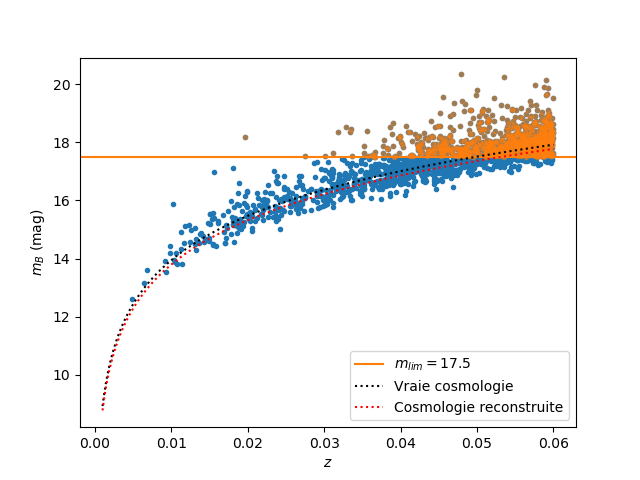
\includegraphics[width=0.8\textwidth]{figures/Malmquist.png}
	\caption{Illustration d'un biais de Malmquist sur une distribution simulée. Un télescope présentant une magnitude limite à 17.5 n'observera pas les SNe marqués en orange, et une analyse ne prenant pas cette effet en compte reconstruira une cosmologie biaisée négativement par rapport à la cosmologie sous-jacente.}
	\label{fig:malmquist}
\end{figure}

Pour modéliser les SNe, \edris se base sur la formule de Tripp (cf \ref{eq:tripp}) et utilise le vecteur de paramètres suivant
\begin{equation}
	Y_i = \pmqty{m_i \\ x_{1,i} \\ c_i} = \pmqty{M_b + \mu(z_i, \Theta) - \alpha x_{1,i} + \beta c_i \\ x_{1,i} \\ c_i} + \pmqty{\varepsilon_i\\0\\0}
\end{equation}
où $m_i$, $x_{1,i}$, $c_i$ et $z_i$ sont la magnitude apparente, le stretch, la couleur et le redshift de la SN $i$, $\mu(z, \theta)$ est le module de distance en fonction du redshift et de la cosmologie de paramètres $\Theta$, $M_b$ est la magnitude absolue et $\varepsilon_i \sim \mcl N(0, \sigma_{int}^2)$ est le bruit causé par la dispersion intrinsèque.

L'effet de la coupure du biais de Malmquist s'exprime alors sous la forme
\begin{equation}
\begin{array}{l}
	Y_i^{obs} = Y_i + \eta_i \qq{si} m_i \leq m_{lim} + \kappa_i \\
	Y_i^{obs} \qq{n'est pas observé sinon}
\end{array}
\end{equation}
où $C$ est la matrice de covariance complète des paramètres $(m_i, x_i, c_i)$, $\eta_i \sim \mcl N(0, C_i)$ est le bruit de mesure, $m_{lim}$ est la magnitude limite du relevé, et $\kappa_i \sim \mcl N(0, \sigma_d^2)$ est la fluctuation due aux conditions d'observations.

L'effet du biais de Malmquist est alors équivalent à l'introduction d'une fonction de sélection sigmoïde en fonction de la magnitude limite sur les données observées, de paramètres $m_{lim}$ et $\sigma_d$.

La log-vraisemblance s'exprime alors sous la forme
\begin{equation}
	\begin{array}{rcl}
		\Gamma & = & -\ln(\abs{C^{-1}}) + \vb r^\dagger C^{-1} \vb  r\\
			& + & \sum_i 2 \ln\qty[\Phi\qty(\frac{m_{lim} - M_b - \mu_i + \alpha x_i - \beta c_i}{\sqrt{\sigma_{int}^2 + \sigma_d^2}})] - 2 \ln\qty[\Phi\qty(\frac{m_{lim} - m_i^{obs}}{\sqrt{\sigma_d^2 + f(C_i)}})]\\
		\text{avec} & & \Phi(x) = \frac{1}{2}(1 + \erf(\frac{x}{\sqrt{2}})) \qq{et} \vb r = \pmqty{m^{obs}\\x_1^{obs} \\ c^{obs}} - \pmqty{M - \mu+ \alpha x_1 - \beta c\\x_1 \\ c}
	\end{array}
\end{equation}
$\Phi(x)$ est la fonction de répartition d'une Gaussienne centrée réduite et $\vb r$ est le vecteur des résidus entre les paramètres ré-estimés et les paramètres observés. Ce sont les deux derniers termes de la log-vraisemblance qui incluent le biais de Malmquist dans l'ajustement des paramètres.

Pour ajuster le modèle $\mu(z, \Theta)$ et réévaluer les paramètres, \edris a nécessité de nombreuses optimisations. Une de ces optimisations a été une implémentation intelligente de la matrice de covariance utilisant le complément de Schur pour l'inverser efficacement. Une deuxième optimisation est l'utilisation de la méthode d'optimisation dite \textit{Hessian-free} décrite dans \cite{martens_deep_2010}, implémentée en \textsc{JAX}. Cette méthode présente l'avantage de ne nécessiter que des calculs de gradients afin de déterminer une approximation de la hessienne, et non de la hessienne complète.


\section{Méthode de l'analyse jointe $f\sigma_8$}
\label{anx:fs8}

Comme mentionné précédemment, l'analyse $f\sigma_8$ se base sur la méthode de comparaison entre les vitesses particulières et celles obtenues à partir du champ de densité, plus précisément sur la méthodologie de \cite{stahl_peculiar-velocity_2021}.

La relation entre le champ de vitesse et le contraste de densité des galaxies $\delta_g = \frac{\rho_g}{\ov{\rho_g}} - 1$ est donné par~:
\begin{equation}
    \vb v (\vb r) = \frac{H_0 \mcl B}{4 \pi} \int_0^{R_{max}} \dd[3]{\vb r'} \delta_g(\vb r') \frac{\vb r' - \vb r}{\abs{\vb r' - \vb r}} + \vb V_{ext}
\end{equation}
où $\mcl B =\frac{f}{b}$, avec $b$ le biais entre le contraste de densité des galaxies et celui de la matière noire ($\delta_g = b \delta_{DM}$), $R_{max}$ est la distance maximale couverte par le catalogue, et $\vb V_{ext}$ est le flux cohérent causé par des structures à l'extérieur du catalogue.

Les vitesses obtenues à partir du champ de densité sont alors ajustées sur celles des vitesses particulières issues des SN à partir d'une méthode \textit{Forward Likelihood}. Les paramètres $\mcl B$ et $\vb V_{ext}$ ainsi que d'autres paramètres de nuisance liés aux observations $\vb \Theta$ (notamment les paramètres du modèle de Tripp $\alpha$, $\beta$, $M_b$ et $\sigma_{int}$, voir Eq. \ref{eq:tripp}) sont reliés aux paramètres observables des SN $\{\vb x_i\}$ via la probabilité conditionnelle $\mcl P(\mcl B, \vb V_{ext}, \vb \Theta | \vb x_i)$, qui peut être exprimée à l'aide du théorème de Bayes (\cite{stahl_peculiar-velocity_2021})
\begin{equation}
    \mcl P(\mcl B, \vb V_{ext}, \vb \Theta | \vb x_i) \propto \mcl P(\vb x_i|\mcl B, \vb V_{ext}, \vb \Theta) \mcl P(\mcl B, \vb V_{ext}, \vb \Theta)
\end{equation}
On cherche donc à reconstruire les distributions contraintes par les observations des paramètres de biais galactique, de flux cohérent, et de nuisance ($\mcl P(\mcl B, \vb V_{ext}, \vb \Theta | \vb x_i)$) à l'aide de la distribution des SN de paramètres  $\vb x_i$ compte tenu du biais galactique, du flux cohérent, et des paramètres de nuisance ($\mcl P(\vb x_i | \mcl B, \vb V_{ext}, \vb \Theta )$)  et d'un prior sur la distributions de ces paramètres ($\mcl P(\mcl B, \vb V_{ext}, \vb \Theta)$).

Les priors sur les paramètres de nuisance du modèle de Tripp sont non restrictifs, ils imposent simplement $\alpha, \beta > 0$ et $M < 0$, tandis que la dispersion intrinsèque $\sigma_{int}$ (cf. Eq. \ref{eq:tripp}) est log-normale avec un pic à $0.15$ mag.

Pour corriger d'éventuelles inhomogénéités selon différentes lignes de visées, on doit introduire de plus une distribution radiale
\begin{equation}
    \mcl P(\vb r|\vb \Theta) = \frac{1}{\mcl N(\vb \Theta)} r^2 \exp{- \frac{\qty[\mu(\vb r) - \mu(\vb\Theta)]^2}{2 \sigma_\mu^2(\vb \Theta)}} \qty[1 + \delta_g(\vb r)]
\end{equation}
où $\vb r$ est un vecteur comobile pointant sur la sphère célèste, $\mcl N(\vb \Theta)$ est un coefficient de normalisation, $\mu$ est le module de distance, et $\sigma_\mu$ est l'erreur sur le module de distance causée par la dispersion intrinsèque des SNe. On obtient alors la vraisemblance suivante
\begin{equation}
    \mcl P(\vb x_i|\mcl B, \vb V_{ext}, \vb \Theta) = \int_0^{R_{max}} \dd{r} \mcl P (\vb x_i|\vb r, \mcl B, \vb V_{ext}, \vb \Theta) \mcl P(\vb r|\vb \Theta)
\end{equation}
avec
\begin{equation}
     \mcl P (\vb x_i|\vb r, \mcl B, \vb V_{ext}, \vb \Theta) = \frac{1}{\sqrt{2 \pi \sigma_\nu^2}} \exp{-\frac{\qty[c z_{obs} - cz_{pred}(\vb r, \mcl B, \vb V_{ext})]^2}{2\sigma_\nu^2}}
\end{equation}
$z_{obs}$ est le redshift observé de la SN, et $z_{pred}$ est la prédiction de ce redshift à partir du redshift cosmologique et des vitesses reconstruites grâce à
\begin{equation}
    1 + z_{pred}(\vb r, \mcl B, \vb V_{ext}) = (1 + z_{cosmo}(\vb r)) \qty[1 + \frac{1}{c} (\mcl B \vb v(r) + \vb V_{ext}) \cdot \vu r]
\end{equation}
$\sigma_\nu$ peut être soit ajusté avec les autres paramètres de nuisance comme dans \cite{stahl_peculiar-velocity_2021}, auquel cas il suit une dispersion gaussienne, soit fixé comme dans \cite{boruah_cosmic_2020}.

Finalement, la log-vraisemblance s'écrit
\begin{equation}
    \mcl L = \ln \mcl P(\mcl B, \vb V_{ext}, \vb \Theta) + \sum_i P(\vb x_i|\mcl B, \vb V_{ext}, \vb \Theta)
\end{equation}
Cette vraisemblance est alors explorée avec une Chaîne de Markov Monte Carlo, et produit des résultats comme ceux de \cite{stahl_peculiar-velocity_2021} représentés en Fig. \ref{fig:stahl}, qui sont en très bon accord avec d'autres analyses $f\sigma_8$ et ont une meilleure précision que les analyses $f\sigma_8$ utilisant seulement les RSD.

\begin{figure}
    \centering
    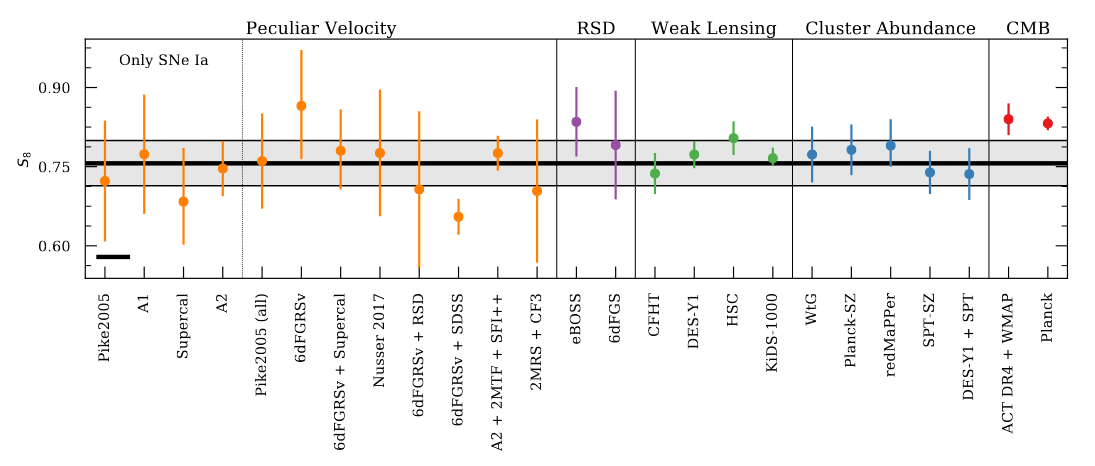
\includegraphics[width=0.8\textwidth]{figures/Stahl_fig_6.png}
    \caption{Paramètre $S_8 = f \sigma_8/(0.3)^{0.55}$ reconstruit par diverses méthodes. Les lignes noires représentent la valeur et l'incertitude de la valeur reconstruite par \cite{stahl_peculiar-velocity_2021}. Crédit : B. Stahl}
    \label{fig:stahl}
\end{figure}


\printbibliography

\end{document}
